\chapter{Coxeter 群与 Tits 系统}

\section{Coxeter 群}

在本节中，W 表示一个用乘法记号书写的群，其单位元为 1；S 表示 W 的一个生成元集合，满足 \(S = S^{-1}\) 且 \(1 \notin S\)。W 的每个元素都是 S 中元素的某个有限序列的乘积。从第 3 号开始，我们假定 S 的每个元素的阶都是 2。

\subsection{长度与约化分解}

定义 1. 设 \(w \in W\)。\(w\) 的长度（相对于 \(S\)），记为 \(l_{S}(w)\) 或简称为 \(l(w)\)，是满足 \(q \geqslant 0\) 且 \(w\) 是由 \(q\) 个 \(S\) 中元素组成的序列的乘积的最小整数。\(w\) 的一个约化分解（相对于 \(S\)）是任意序列 \(s = (s_1, \ldots, s_q)\)，其元素属于 \(S\)，满足 \(w = s_1 \ldots s_q\) 且 \(q = l(w)\)。

因此，1 是长度为 0 的唯一元素，而 \(S\) 由长度为 1 的元素组成。

命题 1. 设 w 和 w' 属于 W。我们有以下公式：

\[
l (w w ^ {\prime}) \leqslant l (w) + l (w ^ {\prime}),\tag{1}
\]

\[
l (w ^ {- 1}) = l (w),\tag{2}
\]

\[
\left| l (w) - l \left(w ^ {\prime}\right) \right| \leqslant l \left(w w ^ {\prime - 1}\right).\tag{3}
\]

设 \((s_{1},\ldots,s_{p})\) 和 \((s_{1}^{\prime},\ldots,s_{q}^{\prime})\) 分别是 w 和 \(w^{\prime}\) 的约化分解。因此 \(l(w)=p\) 且 \(l(w^{\prime})=q\) 。由于 \(ww^{\prime}=s_{1}\ldots s_{p}s_{1}^{\prime}\ldots s_{q}^{\prime}\)，有 \(l(ww^{\prime})\leqslant p+q\)，这就证明了 (1)。由于 \(S=S^{-1}\) 且 \(w^{-1}=s_{p}^{-1}\ldots s_{1}^{-1}\)，有 \(l(w^{-1})\leqslant p=l(w)\)。用 \(w^{-1}\) 代替 w，得到相反的不等式 \(l(w)\leqslant l(w^{-1})\)，从而证明 (2)。在 (1) 和 (2) 中以 \(ww^{\prime-1}\) 代替 w，得到关系

\[
l (w) - l \left(w ^ {\prime}\right) \leqslant l \left(w w ^ {\prime - 1}\right),\tag{4}
\]

\[
l \left(w w ^ {\prime - 1}\right) = l \left(w ^ {\prime} w ^ {- 1}\right).\tag{5}
\]

在 (4) 中交换 \(w\) 和 \(w'\)，由 (5) 得到 \(l(w') - l(w) \leqslant l(ww'^{-1})\)，从而证明 (3)。

推论。设 \(\mathbf{s} = (s_{1}, \ldots, s_{p})\) 和 \(\mathbf{s}' = (s_{1}', \ldots, s_{q}')\) 是 S 中元素的两个序列，满足 \(w = s_{1} \ldots s_{p}\) 且 \(w' = s_{1}' \ldots s_{q}'\)。如果序列 \((s_{1}, \ldots, s_{p}, s_{1}', \ldots, s_{q}')\) 是 \(ww'\) 的一个约化分解，则 s 是 w 的一个约化分解，而 \(s'\) 是 \(w'\) 的一个约化分解。

根据假设，\(l(w) \leqslant p\)，\(l(w') \leqslant q\)，且 \(l(ww') = p + q\)。由 (1)，必有 \(l(w) = p\) 且 \(l(w') = q\)，于是得到该推论。

备注。由公式 (1) 和 (2)，公式 \(d(w, w') = l(ww'^{-1})\) 在 W 上定义了一个距离，该距离在右平移下不变。

\subsection{二面体群}

定义 2. 二面体群是由两个不同的二阶元素生成的群。

例。设 M 为乘法群 \(\{1,-1\}\)，并设 m 是一个 \(\geqslant2\) 或 \(m=\infty\) 的整数。于是 M 通过 \((-1).x=-x\) 作用于群 Z/mZ（分别地，作用于 Z），相应的 M 与 Z/mZ（分别地，M 与 Z）的半直积记为 \(D_{m}\)。因此，\(D_{m}\) 的元素是形如 \((\varepsilon,x)\) 的对，其中 \(\varepsilon=\pm1\) 且 \(x\in Z/mZ\)（分别地，\(x\in Z\)）；\(D_{m}\) 上的群运算由公式

\[
(\varepsilon , x). (\varepsilon^ {\prime}, x ^ {\prime}) = (\varepsilon \varepsilon^ {\prime}, \varepsilon^ {\prime} x + x ^ {\prime}).\tag{6}
\]

我们把 \(\iota\) 记作模 \(m\) 的 1 的剩余类（分别地，\(\iota = 1\)），并置

\[
\rho = (- 1, 0), \quad \rho^ {\prime} = (- 1, \iota), \quad \pi = (1, \iota).\tag{7}
\]

于是 \(\rho^2 = \rho'^2 = 1\) 且 \(\pi = \rho \rho'\)。公式

\[
\pi^ {n} = (1, n \iota), \quad \rho \pi^ {n} = (- 1, n \iota)\tag{8}
\]

表明 \(D_{m}\) 是由 \(\{\rho,\rho'\}\) 生成的二面体群。

命题 2. 假设 \(S\) 由两个不同的二阶元素 \(s\) 和 \(s'\) 组成。

\begin{enumerate}
\def\labelenumi{(\roman{enumi})}
\item
  由 \(p = ss'\) 生成的 W 的子群 P 是正规子群，且 W 是子群 \(T = \{1, s\}\) 与 P 的半直积。此外，\((W : P) = 2\)。
\item
  令 \(m\) 为 \(p\) 的阶（有限或无限）。则 \(m \geqslant 2\)，且 \(W\) 的阶为 \(2m\)。存在唯一同构 \(\varphi\)，从 \(D_m\) 到 \(W\)，满足 \(\varphi(\rho) = s\) 且 \(\varphi(\rho') = s'\)。
\item
  我们有 \(sps^{-1} = sss's = s's = p^{-1}\)，因而
\end{enumerate}

\[
s p ^ {n} s ^ {- 1} = p ^ {- n}\tag{9}
\]

对每个整数 \(n\) 都成立。由于 \(W\) 由 \(\{s, s'\}\) 生成，因而也由 \(\{s, p\}\) 生成，子群 \(P\) 是正规子群。因此 \(TP\) 是 \(W\) 的一个子群；由于 \(TP\) 包含 \(s\) 和 \(s' = sp\)，有 \(W = TP = P \cup sP\)。为了证明 (i)，因此只需证明 \(W \neq P\)。若 \(W = P\)，则群 \(W\) 是交换群，所以 \(p^2 = s^2 s'^2 = 1\)。但此时 \(W = P\) 中只有 1 和 \(p\) 两个元素，这与 \(W\) 至少包含三个元素（即 1、\(s\) 和 \(s'\)）的假设矛盾。

\begin{enumerate}
\def\labelenumi{(\roman{enumi})}
\setcounter{enumi}{1}
\tightlist
\item
  由于 \(s \neq s'\)，有 \(p \neq 1\)，故 \(m \geqslant 2\)。由于 P 的阶为 m 且 (W : P) = 2，W 的阶为 2m。当 m 有限（分别地，无限）时，存在一个同构 \(\varphi'\)，从 Z/mZ（分别地，Z）到 P，将 \(\pi\) 映到 p。~此外，存在一个同构 \(\varphi''\)，从 M = \{1, -1\} 到 T，将 -1 映到 s。群 W 是 T 与 P 的半直积。根据公式 (9) 以及 \(\rho\pi^{n}\rho^{-1} = \pi^{-n}\)，\(\varphi'\) 和 \(\varphi''\) 诱导出同构 \(\varphi\)，从 D\_\{m\} 到 W，满足 \(\varphi(\rho) = s\) 和 \(\varphi(\pi) = p\)，从而 \(\varphi(\rho') = s'\)。\(\varphi\) 的唯一性由 D\_\{m\} 由 \(\{\rho, \rho'\}\) 生成这一事实得到。
\end{enumerate}

备注。考虑一个阶为 2m、由两个不同的二阶元素 s 和 \(s'\) 生成的二面体群 W。记 \(s_{q}\)（分别地，\(s'_{q}\)）为长度为 q 的序列，其编号为奇数（分别地，偶数）的项等于 s，而编号为偶数（分别地，奇数）的项等于 \(s'\)；并记 \(w_{q}\)（分别地，\(w'_{q}\)）为序列 \(s_{q}\)（分别地，\(s'_{q}\)）的乘积。我们有

\[
\begin{array}{r l} w _ {2 k} = (s s ^ {\prime}) ^ {k}, & w _ {2 k + 1} = (s s ^ {\prime}) ^ {k} s, \\ w _ {2 k} ^ {\prime} = (s ^ {\prime} s) ^ {k} = (s s ^ {\prime}) ^ {- k}, & w _ {2 k + 1} ^ {\prime} = (s ^ {\prime} s) ^ {k} s ^ {\prime} = (s s ^ {\prime}) ^ {- k - 1} s. \end{array}
\]

如果 \(\mathbf{s} = (s_1, \ldots, s_q)\) 是关于 \(\{s, s'\}\) 的 W 中元素 \(w\) 的一个约化分解，那么显然 \(s_i \neq s_{i+1}\)，其中 \(1 \leqslant i \leqslant q-1\)。因此，\(\mathbf{s} = \mathbf{s}_q\) 或 \(\mathbf{s} = \mathbf{s}_q'\)。

若 \(m = \infty\)，则 \((ss')^n\) 和 \((ss')^ns\) 对于 \(n \in \mathbf{Z}\) 彼此不同。因此，\(w_q\)（\(q \geqslant 0\)）和 \(w_q'\)（\(q > 0\)）彼此不同；若 \(\mathbf{s}\) 是 \(w_q\)（分别地，\(w_q'\)）的一个约化分解，则必有 \(\mathbf{s} = \mathbf{s}_q\)（分别地，\(\mathbf{s} = \mathbf{s}_q'\)）。由此可得 \(l(w_q) = l(w_q') = q\)，且 \(\mathbf{W}\) 中元素的约化分解集合由 \(\mathbf{s}_q\) 和 \(\mathbf{s}_q'\) 组成。此外，\(\mathbf{W}\) 的每个元素都有唯一的约化分解。

现在设 \(m\) 有限。若 \(q \geqslant 2m\)，则 \(w_{q} = w_{q - 2m}\) 且 \(w_{q}' = w_{q - 2m}'\)；若 \(m \leqslant q \leqslant 2m\)，则 \(w_{q} = w_{2m - q}'\)，\(w_{q}' = w_{2m - q}\)。因此，\(\mathbf{s}_q\) 和 \(\mathbf{s}_q'\) 在 \(q > m\) 时都不是约化分解。由此可知，\(2m\) 个元素 \(W\) 中的每一个，都是以下 \(2m\) 个元素之一：\(w_0 = w_0'\)、\(w_q\) 和 \(w_q'\)（其中 \(1 \leqslant q \leqslant m - 1\)），以及 \(w_m = w_m'\)。因此这 \(2m\) 个元素彼此不同，并且如上所述，\(l(w_q) = l(w_q') = q\) 当 \(q \leqslant m\) 时成立，而 \(W\) 中元素的约化分解集合由 \(s_q\) 和 \(s_q'\)（当 \(0 \leqslant q \leqslant m\) 时）组成。\(W\) 中除 \(w_m\) 外的每个元素都有唯一的约化分解；\(w_m\) 有两个。

\subsection{Coxeter 群的基本性质}

回顾一下，从现在起我们假定 S 的元素的阶都是 2。

定义 3. 如果 (W,S) 满足下述条件，则称 (W,S) 为 Coxeter 系统：

\begin{enumerate}
\def\labelenumi{(\Alph{enumi})}
\setcounter{enumi}{2}
\tightlist
\item
  对于 \(s, s'\) 属于 \(S\)，令 \(m(s, s')\) 为 \(ss'\) 的阶，并令 \(I\) 为对 \((s, s')\) 的集合，其中 \(m(s, s')\) 有限。生成集 \(S\) 以及关系 \((ss')^{m(s, s')} = 1\)（对于 \((s, s')\) 属于 \(I\)）构成一个表示 \(^{1}\)，其对应的群为 \(W\)。
\end{enumerate}

当 (W,S) 是 Coxeter 系统时，也常常滥用语言称 W 为 Coxeter 群。

例子。1) 设 \(m\) 是一个 \(\geqslant 2\) 或 \(\infty\) 的整数，并设 \(W\) 是由生成元集合 \(S = \{s, s'\}\) 以及下列关系定义的群：关系包括 \(s^2 = s'^2 = 1\)（当 \(m = \infty\) 时）以及 \(s^2 = s'^2 = (ss')^m = 1\)（当 \(m\) 有限时）。另一方面，考虑二面体群 \(D_m\)（第 2 号，例）以及由 (7) 定义的元素 \(\rho\) 和 \(\rho'\)，它们属于 \(D_m\)。由于 \(\rho^2 = \rho'^2 = 1\)，并且 \((\rho \rho')^m = 1\) 当 \(m\) 有限时，存在唯一同态 \(f\)，从 \(W\) 到 \(D_m\)，使得 \(f(s) = \rho\) 且 \(f(s') = \rho'\)。由于 \(\rho \rho'\) 的阶为 \(m\)，故 \(ss'\) 本身的阶为 \(m\)。因此，\((W, S)\) 是一个 Coxeter 系统，\(W\) 是阶为 \(2m\) 的二面体群，而 \(f\) 是同构（命题 2）。

通过结构传递，得到每个二面体群都是 Coxeter 群。

\begin{enumerate}
\def\labelenumi{\arabic{enumi})}
\setcounter{enumi}{1}
\item
  设 \(\mathfrak{S}_n\) 为次数 \(n\) 的对称群，其中 \(n \geqslant 2\)。设 \(s_i\) 为 \(i\) 与 \(i + 1\) 的换位，其中 \(1 \leqslant i < n\)，并设 \(S = \{s_1, \ldots, s_{n-1}\}\)。可证明（§2，第 4 号，例以及 §1，习题 4），\((\mathfrak{S}_n, S)\) 是一个 Coxeter 系统。
\item
  关于有限 Coxeter 群的分类，参见第 4 章，第 4 节。
\end{enumerate}

备注。设 \((W,S)\) 是一个 Coxeter 系统。存在一个同态 \(\varepsilon\)，从 W 到群 \(\{1,-1\}\)，其特征为 \(\varepsilon(s)=-1\)，对所有 \(s\in S\)。我们称 \(\varepsilon(w)\) 为 w 的符号；它等于 \((-1)^{l(w)}\)。因此，公式 \(\varepsilon(ww')=\varepsilon(w)\varepsilon(w')\) 转化为 \(l(ww')\equiv l(w)+l(w')\) mod. 2。

命题 3. 假设 (W, S) 是一个 Coxeter 系统。于是，S 中的两个元素 s 和 s' 在 W 中共轭 \(^{2}\)，当且仅当满足下述条件：

\begin{enumerate}
\def\labelenumi{(\Roman{enumi})}
\tightlist
\item
  存在一个有限序列 \((s_1, \ldots, s_q)\)，其元素属于 \(S\)，使得 \(s_1 = s, s_q = s'\)，且 \(s_j s_{j+1}\) 的阶在 \(1 \leqslant j < q\) 时为有限奇数。
\end{enumerate}

设 \(s\) 和 \(s'\) 属于 \(S\)，使得 \(p = ss'\) 的阶为有限数 \(2n + 1\)。由 (9)，\(sp^{-n} = p^n s\)，因而

\[
p ^ {n} s p ^ {- n} = p ^ {n} p ^ {n} s = p ^ {- 1} s = s ^ {\prime} s s = s ^ {\prime},\tag{10}
\]

且 \(s'\) 与 \(s\) 共轭。

对所有 s 属于 S，令 \(A_{s}\) 为满足 (I) 的 \(s' \in S\) 的集合。根据 (I) 的假设，上述结果表明 \(s_{j}\) 和 \(s_{j+1}\) 在 \(1 \leqslant j < q\) 时共轭，因而每个元素 \(s'\) 属于 \(A_{s}\) 都与 s 共轭。

令 \(f\) 为从 \(S\) 到 \(M = \{1, -1\}\) 的映射，它在 \(A_s\) 上取值 1，在 \(S - A_s\) 上取值 -1。设 \(s'\) 和 \(s''\) 是 \(S\) 中满足 \(s's''\) 的阶为有限数 \(m\) 的元素。则 \(f(s')f(s'') = 1\)，当 \(s'\) 和 \(s''\) 都属于 \(A_s\)，或都属于 \(S - A_s\)。在另一种情形下，\(f(s')f(s'') = -1\)，但 \(m\) 为偶数。因此，在所有情形下，\((f(s')f(s''))^m = 1\)。由于 \((W, S)\) 是 Coxeter 系统，存在一个同态 \(g\)，从 \(W\) 到 \(M\)，诱导出 \(f\)（作用于 \(S\)）。令 \(s'\) 是 \(s\) 的一个共轭元。由于 \(s\) 属于 \(g\) 的核，\(s'\) 也属于其核，因而 \(f(s') = g(s') = 1\)，最后 \(s' \in A_s\)。证毕。

\subsection{Coxeter 群中的约化分解}

设 \((W,S)\) 是一个 Coxeter 系统。令 T 为 W 中 S 的元素的共轭元组成的集合。对于 S 中元素的任意有限序列 \(\mathbf{s}=(s_{1},\ldots,s_{q})\)，记 \(\Phi(\mathbf{s})\) 为由 T 中元素组成的序列 \((t_{1},\ldots,t_{q})\)，其中

\[
t _ {j} = \left(s _ {1} \dots s _ {j - 1}\right) s _ {j} \left(s _ {1} \dots s _ {j - 1}\right) ^ {- 1} \quad \text { for } 1 \leqslant j \leqslant q.\tag{11}
\]

于是 \(t_1 = s_1\)，且 \(s_1 \ldots s_q = t_q t_{q-1} \ldots t_1\)。对于任意元素 \(t \in \mathbf{T}\)，记 \(n(\mathbf{s}, t)\) 为这样的整数 \(j\) 的个数：\(1 \leqslant j \leqslant q\) 且 \(t_j = t\)。最后，置

\[
R = \{1, - 1 \} \times T.
\]

引理 1. (i) 设 \(w \in \mathbf{W}\) 且 \(t \in \mathbf{T}\)。数 \((-1)^{n(\mathbf{s},t)}\) 取同一个值 \(\eta(w,t)\)，对所有序列 \(\mathbf{s} = (s_1, \ldots, s_q)\)（其元素属于 \(S\)）且满足 \(w = s_1 \ldots s_q\) 的情形都如此。

\begin{enumerate}
\def\labelenumi{(\roman{enumi})}
\setcounter{enumi}{1}
\tightlist
\item
  对于 \(w \in \mathbf{W}\)，令 \(\mathrm{U}_w\) 为从 \(\mathbf{R}\) 到自身的如下映射：
\end{enumerate}

\[
\mathrm{U} _ {w} (\varepsilon , t) = (\varepsilon . \eta (w ^ {- 1}, t), w t w ^ {- 1}) \quad (\varepsilon = \pm 1, t \in \mathrm{T}).\tag{12}
\]

映射 \(w \mapsto \mathrm{U}_w\) 是从 \(\mathbf{W}\) 到 \(\mathbb{R}\) 的置换群的一个同态。

对于 \(s \in S\)，定义 \(U_s\) 为从 \(R\) 到自身的映射：

\[
\mathrm{U} _ {s} (\varepsilon , t) = \left(\varepsilon . (- 1) ^ {\delta_ {s, t}}, s t s ^ {- 1}\right) \quad (\varepsilon = \pm 1, t \in \mathrm{T}),\tag{13}
\]

其中 \(\delta_{s,t}\) 是 Kronecker 符号。立即可见 \(U_{s}^{2} = Id_{R}\)，这表明 \(U_{s}\) 是 R 的一个置换。

设 \(\mathbf{s} = (s_1, \ldots, s_q)\) 是由 \(S\) 中元素组成的序列。置 \(w = s_q \ldots s_1\) 且 \(U_{\mathbf{s}} = U_{s_q} \ldots U_{s_1}\)。我们将对 \(q\) 作归纳证明：

\[
\mathrm{U} _ {\mathbf {s}} (\varepsilon , t) = (\varepsilon . (- 1) ^ {n (\mathbf {s}, t)}, w t w ^ {- 1}).\tag{14}
\]

当 \(q = 0,1\) 时这是显然的。若 \(q > 1\)，置 \(\mathbf{s}' = (s_1,\dots ,s_{q - 1})\)，并置

\[
w ^ {\prime} = s _ {q - 1} \dots s _ {1}.
\]

利用归纳假设，得到

\[
\begin{array}{r l} \mathrm{U} _ {\mathbf {s}} (\varepsilon , t) & = \mathrm{U} _ {s _ {q}} (\varepsilon . (- 1) ^ {n (\mathbf {s} ^ {\prime}, t)}, w ^ {\prime} t w ^ {\prime - 1}) \\ & = (\varepsilon . (- 1) ^ {n (\mathbf {s} ^ {\prime}, t) + \delta_ {s _ {q}, w ^ {\prime} t w ^ {\prime - 1}}}, w t w ^ {- 1}). \end{array}
\]

但是 \(\Phi(\mathbf{s}) = (\Phi(\mathbf{s}'), w'^{-1}s_q w')\)，且 \(n(\mathbf{s}, t) = n(\mathbf{s}', t) + \delta_{w'^{-1}s_q w', t}\)，这就证明了公式 (14)。

现在设 \(s, s' \in S\)，满足 \(p = ss'\) 的阶为有限数 \(m\)。令 \(\mathbf{s} = (s_1, \ldots, s_{2m})\) 为由 \(S\) 中元素按下述方式定义的序列：满足 \(s_j = s\)（当 \(j\) 为奇数）且 \(s_j = s'\)（当 \(j\) 为偶数）。于是 \(s_{2m} \ldots s_1 = p^{-m} = 1\)，公式 (11) 蕴含

\[
t _ {j} = p ^ {j - 1} s \quad \text { for } 1 \leqslant j \leqslant 2 m.\tag{15}
\]

由于 \(p\) 的阶为 \(m\)，元素 \(t_1, \ldots, t_m\) 彼此不同，且 \(t_{j+m} = t_j\) 对 \(1 \leqslant j \leqslant m\) 成立。对于所有 \(t \in \mathbf{T}\)，整数 \(n(\mathbf{s}, t)\) 因而等于 0 或 2，且 (14) 表明 \(\mathrm{U_s} = \mathrm{Id_R}\)。换言之，\((\mathrm{U_sU_{s'}})^m = \mathrm{Id_R}\)。因此，根据 Coxeter 系统的定义，存在一个同态 \(w \mapsto \mathrm{U}_w\)，从 \(W\) 到 \(R\) 的置换群，使得 \(U_s\) 由 (13) 的右端给出。于是 \(U_w = U_s\)，其中每个序列 \(s = (s_1, \ldots, s_q)\) 都满足 \(w = s_q \ldots s_1\)，引理 1 立即由 (14) 得出。

引理 2. 设 \(\mathbf{s} = (s_1, \ldots, s_q)\)，\(\Phi(\mathbf{s}) = (t_1, \ldots, t_q)\)，且 \(w = s_1 \ldots s_q\)。令 \(\mathrm{T}_w\) 为 \(\mathrm{T}\) 中满足 \(\eta(w, t) = -1\) 的元素集合。则 \(\mathbf{s}\) 是 \(w\) 的一个约化分解，当且仅当 \(t_i\) 彼此不同；在此情形下，\(\mathrm{T}_w = \{t_1, \ldots, t_q\}\)，且 \(\operatorname{Card}(\mathrm{T}_w) = l(w)\)。

显然 \(T_{w} \subset \{t_{1}, \ldots, t_{q}\}\)。取 s 为约化分解，便得到 \(\operatorname{Card}(T_{w}) \leqslant l(w)\)。此外，若 \(t_{i}\) 彼此不同，则 \(n(\mathbf{s}, t)\) 根据 t 是否属于 \(\{t_{1}, \ldots, t_{q}\}\) 分别等于 1 或 0。由此得到 \(T_{w} = \{t_{1}, \ldots, t_{q}\}\)，并且 \(q = \operatorname{Card}(T_{w}) \leqslant l(w)\)，这说明 s 是约化的。最后，若 \(t_{i} = t_{j}\)，且 i \textless{} j，则有 \(s_{i} = us_{j}u^{-1}\)，其中 \(u = s_{i+1} \ldots s_{j-1}\)，因而

\[
w = s _ {1} \dots s _ {i - 1} s _ {i + 1} \dots s _ {j - 1} s _ {j + 1} \dots s _ {q}.
\]

这表明 s 不是 w 的约化分解。

引理 3. 设 \(w \in \mathbb{W}\) 且 \(s \in \mathbb{S}\)，满足 \(l(sw) \leqslant l(w)\)。对于任意序列 \(\mathbf{s} = (s_1, \ldots, s_q)\)，其元素属于 \(\mathbb{S}\) 且满足 \(w = s_1 \ldots s_q\)，存在一个整数 \(j\)，满足 \(1 \leqslant j \leqslant q\)，并且

\[
s s _ {1} \dots s _ {j - 1} = s _ {1} \dots s _ {j - 1} s _ {j}.
\]

令 \(p\) 为 \(w\) 的长度，并令 \(w' = sw\)。由第 3 号的备注，\(l(w') \equiv l(w) + 1 \mod 2\)。假设 \(l(w') \leqslant l(w)\)，再结合关系

\[
| l (w) - l (w ^ {\prime}) | \leqslant l (w w ^ {\prime - 1}) = l (s) = 1
\]

从而得到 \(l(w') = p - 1\)。取一个约化分解

\[
\left(s _ {1} ^ {\prime}, \ldots , s _ {p - 1} ^ {\prime}\right)
\]

它是 \(w'\) 的约化分解，并置 \(\mathbf{s} = (s, s_1', \ldots, s_{p-1}')\) 和 \(\Phi(\mathbf{s}') = (t_1', \ldots, t_p')\)。显然，\(\mathbf{s}'\) 是 \(w\) 的一个约化分解，且 \(t_1' = s\)。根据引理 2，元素 \(t_1', \ldots, t_p'\) 彼此不同，故 \(n(\mathbf{s}', s) = 1\)。由于 \(w\) 是序列 \(\mathbf{s}\) 的乘积，根据引理 1，\(n(\mathbf{s}, s) \equiv n(\mathbf{s}', s) \mod 2\)，从而 \(n(\mathbf{s}, s) \neq 0\)。因此，\(s\) 等于某个元素 \(t_j\)，而该元素属于序列 \(\Phi(\mathbf{s})\)，于是引理得证。

备注。引理 2 中定义的集合 \(T_{w}\) 由形如 \(w''sw''^{-1}\) 的元素组成，这些元素对应于三元组 \((w', w'', s) \in W \times W \times S\)，满足 \(w = w''sw'\) 且 \(l(w') + l(w'') + 1 = l(w)\)。

\subsection{交换条件}

``交换条件''是关于 (W, S) 的如下断言：

\begin{enumerate}
\def\labelenumi{(\Alph{enumi})}
\setcounter{enumi}{4}
\tightlist
\item
  设 \(w \in W\) 和 \(s \in S\) 满足 \(l(sw) \leqslant l(w)\)。对于任意约化分解 \((s_1, \ldots, s_q)\) 的 \(w\)，存在整数 \(j\)，满足 \(1 \leqslant j \leqslant q\)，并且
\end{enumerate}

\[
s s _ {1} \dots s _ {j - 1} = s _ {1} \dots s _ {j - 1} s _ {j}.\tag{16}
\]

在本号中，我们假定 \((W,S)\) 满足 (E)。由引理 3，当 \((W,S)\) 是 Coxeter 系统时，这一条件成立。因此，本号的结果适用于 Coxeter 系统。

命题 4. 设 \(s \in S\)、\(w \in W\)，且 \(s = (s_1, \ldots, s_q)\) 是 \(w\) 的一个约化分解。则下列两种情形必有一种成立：

\begin{enumerate}
\def\labelenumi{\alph{enumi})}
\item
  \(l(sw) = l(w) + 1\)，且 \((s, s_1, \ldots, s_q)\) 是 sw 的一个约化分解。
\item
  \(l(sw) = l(w) - 1\)，并且存在整数 \(j\)，满足 \(1 \leqslant j \leqslant q\)，\((s_1, \ldots, s_{j-1}, s_{j+1}, \ldots, s_q)\) 是 \(sw\) 的一个约化分解，而 \((s, s_1, \ldots, s_{j-1}, s_{j+1}, \ldots, s_q)\) 是 \(w\) 的一个约化分解。
\end{enumerate}

置 \(w' = sw\)。由第 1 号的公式 (3)，有

\[
\left| l (w) - l \left(w ^ {\prime}\right) \right| \leqslant l (s) = 1.
\]

我们区分两种情形：

\begin{enumerate}
\def\labelenumi{\alph{enumi})}
\tightlist
\item
  \(l(w') > l(w)\)。于是 \(l(w') = q + 1\) 且 \(w' = ss_1 \ldots s_q\)，所以
\end{enumerate}

\[
\left(s, s _ {1}, \ldots , s _ {q}\right)
\]

是 \(w'\) 的一个约化分解。

\begin{enumerate}
\def\labelenumi{\alph{enumi})}
\setcounter{enumi}{1}
\tightlist
\item
  \(l(w') \leqslant l(w)\)。由 (E)，存在整数 \(j\)，满足 \(1 \leqslant j \leqslant q\)，且 (16) 成立。于是 \(w = ss_1 \ldots s_{j-1}s_{j+1} \ldots s_q\)，从而
\end{enumerate}

\[
w ^ {\prime} = s _ {1} \dots s _ {j - 1} s _ {j + 1} \dots s _ {q}.
\]

由于 \(q - 1 \leqslant l(w') \leqslant q\)，可知 \(l(w') = q - 1\)，且 \((s_1, \ldots, s_{j-1}, s_{j+1}, \ldots, s_q)\) 是 \(w'\) 的一个约化分解。

引理 4. 设 \(w \in W\) 的长度为 \(q \geqslant 1\)，令 \(D\) 为 \(w\) 的约化分解集合，并令 \(F\) 为从 \(D\) 到集合 \(E\) 的映射。假设 \(F(s) = F(s')\)，其中 \(s = (s_1, \ldots, s_q)\)、\(s' = (s_1', \ldots, s_q')\) 是 \(D\) 中满足下列某一假设的元素：

\[
a) s _ {1} = s _ {1} ^ {\prime} \text {   or   } s _ {q} = s _ {q} ^ {\prime}.
\]

\begin{enumerate}
\def\labelenumi{\alph{enumi})}
\setcounter{enumi}{1}
\tightlist
\item
  存在 \(s\) 和 \(s'\)，属于 \(S\)，使得 \(s_j = s'_k = s\) 且 \(s_k = s'_j = s'\)，其中 \(j\) 为奇数且 \(k\) 为偶数。
\end{enumerate}

则 F 为常值映射。

\begin{enumerate}
\def\labelenumi{\Alph{enumi})}
\item
  设 \(\mathbf{s}, \mathbf{s}' \in D\)，并置 \(\mathbf{t} = (s_1', s_1, \ldots, s_{q-1})\)。我们将证明：若 \(\mathrm{F}(\mathbf{s}) \neq \mathrm{F}(\mathbf{s}')\)，则 \(\mathbf{t} \in D\) 且 \(\mathrm{F}(\mathbf{t}) \neq \mathrm{F}(\mathbf{s})\)。事实上，\(w = s_1' \ldots s_q'\)，因而 \(s_1' w = s_2' \ldots s_q'\) 的长度为 \(< q\)。由命题 4，存在整数 \(j\)，满足 \(1 \leqslant j \leqslant q\)，使序列 \(\mathbf{u} = (s_1', s_1, \ldots, s_{j-1}, s_{j+1}, \ldots, s_q)\) 属于 D。有 \(\mathrm{F}(\mathbf{u}) = \mathrm{F}(\mathbf{s}')\)，根据条件 \(a\)；若 \(j \neq q\)，同理有 \(\mathrm{F}(\mathbf{s}) = \mathrm{F}(\mathbf{u})\)，从而 \(\mathrm{F}(\mathbf{s}) = \mathrm{F}(\mathbf{s}')\)，这与假设矛盾。因此 \(j = q\)，于是 \(\mathbf{t} = \mathbf{u} \in D\)，且 \(\mathrm{F}(\mathbf{t}) = \mathrm{F}(\mathbf{s}') \neq \mathrm{F}(\mathbf{s})\)。
\item
  设 \(\mathbf{s}\) 和 \(\mathbf{s}'\) 属于 D。对于任意整数 \(j\)，满足 \(0 \leqslant j \leqslant q + 1\)，定义一个序列 \(\mathbf{s}_j\)，由 S 中的 \(q\) 个元素组成，如下：
\end{enumerate}

\[
\begin{array}{r l} \mathbf {s} _ {0} & = (s _ {1} ^ {\prime}, \dots , s _ {q} ^ {\prime}) \\ \mathbf {s} _ {1} & = (s _ {1}, \dots , s _ {q}) \\ \mathbf {s} _ {q + 1 - k} & = (s _ {1}, s _ {1} ^ {\prime}, \dots , s _ {1}, s _ {1} ^ {\prime}, s _ {1}, s _ {2}, \dots , s _ {k}) \\ & \text {for } q - k \text { even and } 0 \leqslant k \leqslant q \end{array}\tag{17}
\]

\[
\mathbf {s} _ {q + 1 - k} = \left(s _ {1} ^ {\prime}, s _ {1}, \ldots , s _ {1}, s _ {1} ^ {\prime}, s _ {1}, s _ {2}, \ldots , s _ {k}\right)
\]

\[
\text { for   } q - k \text {   odd   and   } 0 \leqslant k \leqslant q.
\]

记 \((\mathrm{H}_{j})\) 表示断言 `` \(s_{j} \in D, s_{j+1} \in D\) 且 \(F(s_{j}) \neq F(s_{j+1})\) ''。由 A)，\((\mathrm{H}_{j}) \Longrightarrow (\mathrm{H}_{j+1})\)，且这对 \(0 \leqslant j < q\) 成立；而根据条件 b)，\((\mathrm{H}_{q})\) 不成立。因此，\((\mathrm{H}_{0})\) 不成立。由于 \(s_{0} = s'\) 且 \(s_{1} = s\)，得到 \(F(s) = F(s')\)。

命题 5. 设 M 为一个幺半群（单位元为 1），f 为从 S 到 M 的映射。对于 \(s, s' \in S\)，令 \(m(s, s')\) 为 \(ss'\) 的阶，并置

\[
a (s, s ^ {\prime}) = \left\{ \begin{array}{l l} (f (s) f (s ^ {\prime})) ^ {l} & \text {if } m(s,s^{\prime}) = 2l,\ l \text { finite} \\ (f (s) f (s ^ {\prime})) ^ {l} f (s) & \text {if } m(s,s^{\prime}) = 2l + 1,\ l \text { finite} \\ 1 & \text {if } m(s,s^{\prime}) = \infty . \end{array} \right.\tag{18}
\]

如果 \(a(s, s') = a(s', s)\) 对 \(s \neq s'\) 属于 \(S\) 的情形都成立，则存在一个映射 \(g\)，从 \(W\) 到 \(M\)，使得

\[
g (w) = f \left(s _ {1}\right) \dots f \left(s _ {q}\right)\tag{19}
\]

对所有 \(w \in \mathbf{W}\) 以及任意约化分解 \((s_1, \ldots, s_q)\) 的 \(w\)，

对于任意 \(w \in W\)，令 \(D_w\) 为 \(w\) 的约化分解集合，并令 \(F_w\) 为从 \(D_w\) 到 \(M\) 的映射，由下式定义：

\[
\mathrm{F} _ {w} (s _ {1}, \dots , s _ {q}) = f (s _ {1}) \dots f (s _ {q}).
\]

我们将按 w 的长度归纳，证明 \(F_{w}\) 为常值，这将证明命题 5。由于 \(l(w) = 0, 1\) 的情形是平凡的，我们假定 \(q \geqslant 2\)，并假定对于满足 \(l(w) < q\) 的元素 w，断言已经得到证明。设 w 的长度为 q，且 \(s, s' \in D_w\)；根据引理 4，只需证明在该引理的 a) 和 b) 两种情形下 \(\mathrm{F}_{w}(\mathbf{s}) = \mathrm{F}_{w}(\mathbf{s}')\)。

\begin{enumerate}
\def\labelenumi{\alph{enumi})}
\tightlist
\item
  公式
\end{enumerate}

\[
\mathrm{F} _ {w} \left(s _ {1}, \dots , s _ {q}\right) = f \left(s _ {1}\right) \mathrm{F} _ {w ^ {\prime \prime}} \left(s _ {2}, \dots , s _ {q}\right) = \mathrm{F} _ {w ^ {\prime}} \left(s _ {1}, \dots , s _ {q - 1}\right) f \left(s _ {q}\right)
\]

当 \(w' = s_1 \ldots s_{q-1}\) 且 \(w'' = s_2 \ldots s_q\) 时，上式以及归纳假设表明：\(F_w(\mathbf{s}) = F_w(\mathbf{s}')\)，若 \(s_1 = s_1'\) 或 \(s_q = s_q'\)。

\begin{enumerate}
\def\labelenumi{\alph{enumi})}
\setcounter{enumi}{1}
\tightlist
\item
  假设存在两个元素 \(s\) 和 \(s'\)，属于 \(S\)，使得 \(s_j = s'_k = s\) 且 \(s_k = s'_j = s'\)，其中 \(j\) 为奇数且 \(k\) 为偶数。只需处理 \(s \neq s'\) 的情形。此时，序列 \(s\) 和 \(s'\) 是 \(w\) 的两个不同约化分解，属于由 \(s\) 和 \(s'\) 生成的二面体群。根据第 2 号备注，\(m\)（即 \(ss'\) 的阶）必为有限数；用该备注的记号，\(s = s_m\) 且 \(s' = s'_m\)。因此，\(F_w(s) = a(s, s')\) 且 \(F_w(s') = a(s', s)\)，于是
\end{enumerate}

\[
\mathrm{F} _ {w} (\mathbf {s}) = \mathrm{F} _ {w} (\mathbf {s} ^ {\prime}).
\]

\subsection{Coxeter 群的刻画}

定理 1. (W,S) 是 Coxeter 系统，当且仅当它满足第 5 号的交换条件 (E)。

第 4 号的引理 3 表明，任意 Coxeter 系统都满足 (E)。

反之，假设 (E) 得到满足。设 G 为一个群，f 为从 S 到 G 的映射，使得 \((f(s)f(s'))^{m}=1\)，只要 s 和 \(s'\) 属于 S 且 \(ss'\) 的阶为有限数 m。由命题 5，存在从 W 到 G 的映射 g，使得

\[
g (w) = f (s _ {1}) \dots f (s _ {q})\tag{20}
\]

只要 \(w = s_{1} \ldots s_{q}\) 的长度为 q，就有上述等式。为了证明 (W,S) 是 Coxeter 系统，只需证明 g 是同态；这由公式

\[
g (s w) = f (s) g (w) \quad \text { for } s \in S, w \in W\tag{21}
\]

因为 S 生成 W。由第 5 号的命题 4，只可能有以下两种情形：

\begin{enumerate}
\def\labelenumi{\alph{enumi})}
\item
  \(l(sw) = l(w) + 1\)：若 \((s_1, \ldots, s_q)\) 是 \(w\) 的一个约化分解，则 \((s, s_1, \ldots, s_q)\) 是 \(sw\) 的一个约化分解，于是 (21)。
\item
  \(l(sw) = l(w) - 1\)：置 \(w' = sw\)；于是 \(w = sw'\) 且 \(l(sw') = l(w') + 1\)。由 a)，\(g(w) = f(s)g(sw)\)，因而 \(f(s)g(w) = g(sw)\)，因为 \((f(s))^{2} = 1\)。
\end{enumerate}

\subsection{划分族}

设 \((\mathrm{W}, S)\) 是一个 Coxeter 系统。对于任意 \(s \in \mathrm{S}\)，令 \(\mathrm{P}_s\) 为 \(w\) 属于 \(\mathrm{W}\) 且满足 \(l(sw) > l(w)\) 的元素集合。我们有以下性质：

\[
(A) \bigcap_ {s \in S} P _ {s} = \{1 \}.
\]

事实上，设 \(w \neq 1\) 属于 \(W\)，且 \((s_1, \ldots, s_q)\) 是 \(w\) 的一个约化分解。则 \(q \geqslant 1\)，而 \((s_2, \ldots, s_q)\) 是 \(s_1w\) 的一个约化分解，因此 \(l(w) = q\) 且 \(l(s_1w) = q - 1\)。所以 \(w \notin P_{s_1}\)。

\begin{enumerate}
\def\labelenumi{(\Alph{enumi})}
\setcounter{enumi}{1}
\tightlist
\item
  对于 \(s\) 属于 \(S\) 的任意情形，集合 \(\mathrm{P}_s\) 和 \(s\mathrm{P}_s\) 构成 \(W\) 的一个划分。
\end{enumerate}

设 \(w \in W\) 且 \(s \in S\)。由第 5 号的命题 4，必须区分两种情形：

\begin{enumerate}
\def\labelenumi{\alph{enumi})}
\item
  \(l(sw) = l(w) + 1\)：于是 \(w \in P_s\)。
\item
  \(l(sw) = l(w) - 1\)：置 \(w' = sw\)，于是 \(w = sw'\)；然后
\end{enumerate}

\[
l (w ^ {\prime}) <   l (s w ^ {\prime})
\]

从而 \(w' \in P_s\)，即 \(w \in sP_s\)。

\begin{enumerate}
\def\labelenumi{(\Alph{enumi})}
\setcounter{enumi}{2}
\tightlist
\item
  设 \(s, s'\) 属于 \(S\)，且 \(w\) 属于 \(W\)。若 \(w \in P_s\) 且 \(ws' \in P_s\)，则 \(sw = ws'\)。
\end{enumerate}

设 \(q\) 为 \(w\) 的长度。由 \(w \in P_s\) 可知 \(l(sw) = q + 1\)；由 \(ws' \in P_s\) 可知 \(l(sws') = l(ws') - 1 \leqslant q\)。由于 \(l(sws') = l(sw) \pm 1\)，最终得到 \(l(ws') = q + 1\) 且 \(l(sws') = q\)。

设 \((s_{1},\ldots,s_{q})\) 是 w 的一个约化分解，并令 \(s_{q+1}=s'\)；于是 \((s_{1},\ldots,s_{q},s_{q+1})\) 是元素 \(ws'\) 的一个长度为 \(q+1\) 的约化分解。由交换条件，存在整数 j，满足 \(1\leqslant j\leqslant q+1\)，使得

\[
s s _ {1} \dots s _ {j - 1} = s _ {1} \dots s _ {j}.\tag{22}
\]

若 \(1 \leqslant j \leqslant q\)，则有 \(sw = s_1 \ldots s_{j-1}s_{j+1} \ldots s_q\)，这与公式 \(l(sw) = q + 1\) 矛盾。因此 \(j = q + 1\)，而公式 (22) 可写成 \(sw = ws'\)。

反过来，我们有以下结果：

命题 6. 设 \((\mathrm{P}_s)_{s\in \mathbb{S}}\) 是 W 的子集族，满足 (C) 以及下列条件：

(A') \(1 \in P_{s}\) 对所有 \(s \in S\) 成立。

(B') 集合 \(P_{s}\) 和 \(sP_{s}\) 对所有 \(s \in S\) 都不相交。

则 (W,S) 是一个 Coxeter 系统，并且 \(P_{s}\) 由满足 \(l(sw) > l(w)\) 的 W 的元素 w 组成。

设 \(s \in S\) 且 \(w \in W\)。有两种可能：

\begin{enumerate}
\def\labelenumi{\alph{enumi})}
\tightlist
\item
  \(w \notin \mathrm{P}_s\)。设 \((s_1, \ldots, s_q)\) 是 \(w\) 的一个约化分解，并且
\end{enumerate}

\[
w _ {j} = s _ {1} \dots s _ {j}
\]

当 \(1 \leqslant j \leqslant q\) 时成立；另置 \(w_0 = 1\)。由于 \(w_0 \in \mathrm{P}_s\)（由 \((\mathrm{A}')\)），而 \(w = w_q\) 不属于 \(\mathrm{P}_s\)，因此存在一个整数 \(j\)，满足 \(1 \leqslant j \leqslant q\)，使得 \(w_{j-1} \in \mathrm{P}_s\)，而 \(w_j = w_{j-1}s_j\) 不属于 \(\mathrm{P}_s\)。由 (C)，

\[
s w _ {j - 1} = w _ {j - 1} s _ {j}.
\]

于是我们证明了公式

\[
s s _ {1} \dots s _ {j - 1} = s _ {1} \dots s _ {j - 1} s _ {j}
\]

这意味着 \(sw = s_1 \ldots s_{j-1}s_{j+1} \ldots s_q\)，且 \(l(sw) < l(w)\)。

\begin{enumerate}
\def\labelenumi{\alph{enumi})}
\setcounter{enumi}{1}
\tightlist
\item
  \(w \in \mathbf{P}_s\)：置 \(w' = sw\)，则由 (B') 有 \(w' \notin \mathbf{P}_s\)。由 a)，有 \(l(sw') < l(w')\)，即 \(l(w) < l(sw)\)。
\end{enumerate}

比较 \(a)\) 和 \(b)\) 可知，\(P_s\) 正好由那些 \(w \in W\) 且满足 \(l(sw) > l(w)\) 的元素组成。交换条件由此得到，因为我们在 \(a)\) 中已经看到了它，于是 (W, S) 是一个 Coxeter 系统（第 6 号的定理 1）。

\subsection{Coxeter 群的子群}

在本号中，我们假定 \((W, S)\) 是一个 Coxeter 系统。对于 S 的任意子集 X，记 \(W_{X}\) 为由 X 生成的 W 的子群。

命题 7. 设 \(w\) 属于 W。存在一个子集 \(S_w\)，它是 \(S\) 的子集，使得 \(\{s_1, \ldots, s_q\} = S_w\) 对任意约化分解 \((s_1, \ldots, s_q)\) 的 \(w\) 都成立。

令 M 为由 S 的子集组成的幺半群，其运算为 \((A,B)\mapsto A\cup B\)；M 的单位元为 \(\varnothing\)。置 \(f(s)=\{s\}\)，其中 \(s\in S\)。我们将对 M 和 f 应用第 5 号的命题 5。~有 \(a(s,s')=\{s,s'\}\)，只要 \(s,s'\) 属于 S 且 \(m(s,s')\) 有限，因此存在一个映射 \(g:w\mapsto S_w\)，从 W 到 M，使得 \(g(w)=f(s_1)\cup\cdots\cup f(s_q)\)，即 \(S_w=\{s_1,\ldots,s_q\}\)，对于任意 \(w\in W\) 和任意约化分解 \((s_1,\ldots,s_q)\) 的 w 都如此。

推论 1. 对于任意子集 \(\mathbf{X}\)，它是 \(\mathbf{S}\) 的子集，\(\mathrm{W}_{\mathbf{X}}\) 作为 \(\mathbf{W}\) 的子群，由元素 \(w\)（属于 \(\mathbf{W}\)）组成，且这些元素满足 \(\mathrm{S}_w \subset \mathbf{X}\)。

若 \(w = s_1 \ldots s_q\)，其中 \(s_1, \ldots, s_q\) 属于 \(S\)，则 \(w^{-1} = s_q \ldots s_1\)；因此

\[
\mathrm{S} _ {w ^ {- 1}} = \mathrm{S} _ {w}.\tag{23}
\]

第 5 号的命题 4 表明，对于 \(S_{sw'} \subset \{s\} \cup S_{w'}\)，其中 \(s \in S\) 且 \(w' \in W\)，从而得到公式

\[
\mathrm{S} _ {w w ^ {\prime}} \subset \mathrm{S} _ {w} \cup \mathrm{S} _ {w ^ {\prime}}\tag{24}
\]

对 w 的长度作归纳即可证明。由 (23) 和 (24)，集合 U 由满足 \(w \in W\) 且 \(S_{w} \subset X\) 的元素组成，是 W 的一个子群；我们有 \(X \subset U \subset W_{X}\)，因此 \(U = W_{X}\)。

推论 2. 对于 S 的任意子集 X，都有 \(W_{X} \cap S = X\)。

这由推论 1 以及公式 \(S_s = \{s\}\)（其中 \(s\) 属于 \(S\)）得出。

推论 3. 集合 S 是 W 的极小生成集。

若 \(X \subset S\) 生成 \(W\)，则 \(W = W_X\)，因而由推论 2 有 \(X = S \cap W_X = S\)。

推论 4. 对于 S 的任意子集 X 以及任意 w 属于 \(W_{X}\)，w 关于 \(W_{X}\) 的生成集 X 的长度等于 \(l_{S}(w)\)。

设 \((s_{1},\ldots,s_{q})\) 是把 w 视为 W 的元素时的一个约化分解。我们有 \(w=s_{1}\ldots s_{q}\)，并且 \(s_{j}\in X\) 对 \(1\leqslant j\leqslant q\) 成立；此外，w 不可能是 \(q^{\prime}<q\) 个属于 \(X\subset S\) 的元素的乘积，这是由 \(q=l_{S}(w)\) 的定义所致。

定理 2. (i) 对于任意子集 \(X\)，它是 \(S\) 的子集，\((W_X, X)\) 是一个 Coxeter 系统。

\begin{enumerate}
\def\labelenumi{(\roman{enumi})}
\setcounter{enumi}{1}
\item
  设 \((\mathrm{X}_i)_{i\in \mathbf{I}}\) 是 S 的子集族。若 \(\mathrm{X} = \bigcap_{i\in \mathbf{I}}\mathrm{X}_i\)，则 \(\mathrm{W_X} = \bigcap_{i\in \mathbf{I}}\mathrm{W}_{\mathrm{X}_i}\)。
\item
  设 \(\mathbf{X}\) 和 \(\mathbf{X}'\) 是 \(\mathbf{S}\) 的两个子集。则 \(\mathrm{W_X} \subset \mathrm{W_{X'}}\)（分别地，\(\mathrm{W_X} = \mathrm{W_{X'}}\)），当且仅当 \(\mathbf{X} \subset \mathbf{X'}\)（分别地，\(\mathbf{X} = \mathbf{X'}\)）。
\end{enumerate}

X 的每个元素的阶都是 2，而 X 生成 \(W_{X}\)。设 \(x \in X\) 且 \(w \in W_{X}\)，满足 \(l_{\mathrm{X}}(xw) \leqslant l_{\mathrm{X}}(w) = q\)。由命题 7 的推论 4，有

\[
l _ {S} (x w) \leqslant l _ {S} (w) = q.
\]

设 \(x_{1},\ldots ,x_{q}\) 是 X 中满足 \(w = x_{1}\dots x_{q}\) 的元素。由于 (W,S) 满足交换条件（第 6 号的定理 1），存在整数 \(j\)，满足 \(1\leqslant j\leqslant q\)，且 \(xx_{1}\ldots x_{j - 1} = x_{1}\ldots x_{j - 1}x_{j}\)。因此，\((\mathrm{W_X},\mathrm{X})\) 满足交换条件，故是一个 Coxeter 系统（第 6 号的定理 1）。这就证明了 (i)。

断言 (ii) 和 (iii) 立即由命题 7 的推论 1 得出。

\subsection{Coxeter 矩阵与 Coxeter 图}

定义 4. 设 I 为一个集合。I 型 Coxeter 矩阵是一个对称方阵 \(\mathrm{M} = (m_{ij})_{i,j\in \mathrm{I}}\)，其元素为整数或 \(+\infty\)，并满足关系

\[
m _ {i i} = 1 \quad \text {   for   all   } i \in \mathrm{I};\tag{25}
\]

\[
m _ {i j} \geqslant 2 \quad \text {   for   } i, j \in I \text {   with   } i \neq j.\tag{26}
\]

I 型 Coxeter 图是（滥用术语而言）如下的一个对：一个图 \(\Gamma^{3}\)，其顶点集为 I；以及从该图的边集到由 \(+\infty\) 和所有 \(\geqslant 3\) 的整数构成的集合的一个映射 f。\(\Gamma\) 称为 Coxeter 图 \((\Gamma, f)\) 的底图。

每个 I 型 Coxeter 矩阵的 Coxeter 图 \((\Gamma, f)\) 都与矩阵 \(M\) 相关联，如下所述：

图 \(\Gamma\) 的顶点集为 I，边集为由 I 中元素组成的二元集合 \(\{i,j\}\) 的集合，其中满足 \(m_{ij} \geqslant 3\)，而映射 \(f\) 将边 \(\{i,j\}\) 关联到 M 中相应的元素 \(m_{ij}\)。

显然，这在 I 型 Coxeter 矩阵集合与 I 型 Coxeter 图集合之间给出了一个双射。

为了帮助读者理解我们的论证，我们常常用表示其底图的图示来表示 I 型 Coxeter 图，并在每条边 \(\{i,j\}\) 旁边或上方写出数值 \(f(\{i,j\})\)。如果这些数等于 3，我们通常省略它们。

若 (W,S) 是一个 Coxeter 系统，则矩阵 \(M = (m(s,s'))_{s,s' \in S}\)，其中 \(m(s,s')\) 是 \(ss'\) 的阶，是 S 型 Coxeter 矩阵，称为 (W,S) 的 Coxeter 矩阵：事实上，\(m(s,s) = 1\)，因为 \(s^2 = 1\) 对所有 \(s \in S\) 成立；且 \(m(s,s') = m(s',s) \geqslant 2\) 当 \(s \neq s'\) 时，因为 \(ss' = (s's)^{-1}\) 且 \(\neq 1\)。与 M 相关联的 Coxeter 图 \((\Gamma, f)\) 称为 (W,S) 的 Coxeter 图。我们注意到，两个顶点 \(s\) 和 \(s'\) 属于 \(\Gamma\) 当且仅当 \(s\) 和 \(s'\) 不交换。例如，阶为 \(2m\) 的二面体群的 Coxeter 矩阵为 \(\begin{pmatrix} 1 & m \\ m & 1 \end{pmatrix}\)，其 Coxeter 图表示为

当 \(m \geqslant 3\) 时（或者

\pandocbounded{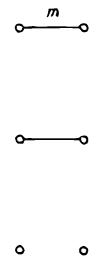
\includegraphics[keepaspectratio]{images/part001_5ff7a109.jpg}}

当 \(m = 3\) 时），而在

当 \(m = 2\) 时。*对称群 \(\mathfrak{S}_n\) 的 Coxeter 图表示为

\pandocbounded{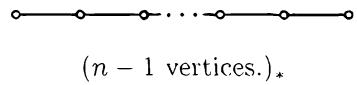
\includegraphics[keepaspectratio]{images/part001_1071b0ee.jpg}}

我们将在后面（第 V 章，第 4 节）证明，反过来，每个 Coxeter 矩阵都是某个 Coxeter 系统的矩阵。

如果 Coxeter 图的底图连通（附录，第 2 号）且非空，则称 Coxeter 系统 \((W,S)\) 是不可约的。等价地，S 非空，并且不存在将 S 划分为两个不同子集 \(S'\) 和 \(S''\) 的划分，使得 \(S'\) 的每个元素都与 \(S''\) 的每个元素交换。更一般地，设 \((\Gamma_{i})_{i\in I}\) 为 \(\Gamma\) 的连通分支族（附录，第 2 号），并设 \(S_{i}\) 为 \(\Gamma_{i}\) 的顶点集。令 \(W_{i}=W_{S_i}\) 为由 \(S_{i}\) 生成的 W 的子群（参见第 8 号）。于是 \((W_{i},S_{i})\) 是不可约 Coxeter 系统（第 8 号，定理 2），称为 \((W,S)\) 的不可约分支。此外，群 W 是限制直积 \(^{4}\)，其因子为子群 \(W_{i}\)（其中 \(i\in I\)）。事实上，这由下面更一般的命题得到：

命题 8. 设 \((\mathrm{S}_{i})_{i\in\mathrm{I}}\) 是 S 的一个划分，使得 \(S_{i}\) 的每个元素都与 \(S_{j}\) 的每个元素交换，只要 \(i\neq j\)。对于所有 \(i\in I\)，令 \(W_{i}\) 为由 \(S_{i}\) 生成的子群。于是 W 是族 \((\mathrm{W}_{i})_{i\in\mathrm{I}}\) 的限制直积。

显然，对于所有 \(i \in I\)，子群 \(W_i'\) 由 \(W_j\)（其中 \(j \neq i\)）的并生成，也由 \(S_i' = \bigcup_{i \neq j} S_j\) 生成。因此

\[
\mathrm{W} _ {i} \cap \mathrm{W} _ {i} ^ {\prime} = \mathrm{W} _ {\varnothing} = \{1 \}
\]

由第 8 号的定理 2。由于 W 由各 \(W_{i}\) 的并生成，命题得证。

\section{Tits 系统}

在本段中，字母 G、B、N、S、T、W 的含义如下文第 1 号所规定。

\subsection{定义与初步性质}

设 G 为一个群，B 为 G 的一个子群。群 \(B \times B\) 通过 \((b, b')\) . \(g = bgb'^{-1}\) 作用在 G 上，其中 \(b, b' \in B\) 且 \(g \in G\)。\(B \times B\) 在 G 上的轨道是当 \(g \in G\) 时的集合 BgB，称为关于 B 的 G 的双陪集。它们构成 G 的一个划分；相应的商记为 B\textbackslash G/B。若 C 和 C' 是双陪集，则 CC' 是双陪集的并。

定义 1. Tits 系统是一个四元组 \((\mathbf{G},\mathbf{B},\mathbf{N},\mathbf{S})\)，其中 \(\mathbf{G}\) 是一个群，\(\mathbf{B}\) 和 \(\mathbf{N}\) 是 \(\mathbf{G}\) 的两个子群，\(\mathbf{S}\) 是 \(\mathrm{N} / (\mathrm{B}\cap \mathrm{N})\) 的一个子集，并满足下列公理：

(T1) 集合 \(\mathrm{B} \cup \mathrm{N}\) 生成 \(\mathrm{G}\)，且 \(\mathrm{B} \cap \mathrm{N}\) 是 \(\mathrm{N}\) 的正规子群。

(T2) 集合 S 生成群 \(W = N/(B \cap N)\)，并且由阶为 2 的元素组成。

(T3) \(sBw \subset BwB \cup BswB\)，其中 \(s \in S\) 且 \(w \in W\)。

(T4) 对所有 \(s \in S\)，都有 \(sBs \not\subset B\)。

群 \(W = N / (B \cap N)\) 有时称为 Tits 系统 \((G, B, N, S)\) 的 Weyl 群。

备注。1) 我们将在第 5 号（定理 3 的推论）看到，如果给定 (G, B, N)，则至多存在一个 N/(B∩N) 的子集 S，使得 (G, B, N, S) 是 Tits 系统。

\begin{enumerate}
\def\labelenumi{\arabic{enumi})}
\setcounter{enumi}{1}
\tightlist
\item
  设 \((G, B, N, S)\) 是一个 Tits 系统，Z 是 G 的包含于 B 中的正规子群。令 \(G' = G/Z, B' = B/Z, N' = N/(Z \cap N)\)，并令 \(S'\) 为 S 在 \(N'/(B' \cap N')\) 中的像。立即可见，\((G', B', N', S')\) 是一个 Tits 系统。
\end{enumerate}

在本段中，设 \((\mathrm{G},\mathrm{B},\mathrm{N},\mathrm{S})\) 为一个 Tits 系统，并置 \(T=B\cap N\)、W=N/T。双陪集均指 G 关于 B 的双陪集。对于任意 \(w\in W\)，置 \(C(w)=BwB\)；这是一个双陪集。

我们将从公理 (T1) 至 (T4) 推出若干初等结论。用 \(w, w', \ldots\) 表示 W 的元素，用 \(s, s', \ldots\) 表示 S 的元素。以下关系是显然的：

\[
\mathrm{C} (1) = \mathrm{B}, \quad \mathrm{C} (w w ^ {\prime}) \subset \mathrm{C} (w). \mathrm{C} (w ^ {\prime}), \quad \mathrm{C} (w ^ {- 1}) = \mathrm{C} (w) ^ {- 1}.\tag{1}
\]

公理 (T3) 也可写成

\[
\mathrm{C} (s). \mathrm{C} (w) \subset \mathrm{C} (w) \cup \mathrm{C} (s w).\tag{2}
\]

此外，由 (1) 有 \(C(sw) \subset C(s).C(w)\)，又因 \(C(s).C(w)\) 是双陪集的并，故只有以下两种可能：

\[
\mathrm{C} (s). \mathrm{C} (w) = \left\{ \begin{array}{l l} \mathrm{C} (s w) & \text {if} \mathrm{C} (w) \not \subset \mathrm{C} (s). \mathrm{C} (w) \\ \mathrm{C} (w) \cup \mathrm{C} (s w) & \text {if} \mathrm{C} (w) \subset \mathrm{C} (s). \mathrm{C} (w). \end{array} \right.\tag{3}
\]

由 (T4)，\(\mathrm{B} \neq \mathrm{C}(s). \mathrm{C}(s)\)；在 (3) 中令 \(w = s\)，并利用关系 \(s^2 = 1\)，得到

\[
\mathrm{C} (s). \mathrm{C} (s) = \mathrm{B} \cup \mathrm{C} (s).\tag{4}
\]

此公式表明，\(B \cup C(s)\) 是 G 的一个子群。将 (4) 两边右乘 \(C(w)\)，并利用公式 (3) 以及关系

\[
\mathrm{B.C} (w) = \mathrm{C} (w),
\]

得到

\[
\mathrm{C} (s). \mathrm{C} (s). \mathrm{C} (w) = \mathrm{C} (w) \cup \mathrm{C} (s w).\tag{5}
\]

对公式 (2)、(3) 和 (5) 中出现的集合取逆，然后以 \(w^{-1}\) 代替 w，得到公式

\[
\mathrm{C} (w). \mathrm{C} (s) \subset \mathrm{C} (w) \cup \mathrm{C} (w s)\tag{(2')}
\]

\[
\mathrm{C} (w). \mathrm{C} (s) = \mathrm{C} (w s) \quad \text {   if   } \mathrm{C} (w) \not \subset \mathrm{C} (w). \mathrm{C} (s)
\]

\[
\mathrm{C} (w). \mathrm{C} (s) = \left\{ \begin{array}{l l} \mathrm{C} (w) \cup \mathrm{C} (w s) & \text {if} \mathrm{C} (w) \subset \mathrm{C} (w). \mathrm{C} (s) \end{array} \right.\tag{3'}
\]

\[
\mathrm{C} (w). \mathrm{C} (s). \mathrm{C} (s) = \mathrm{C} (w) \cup \mathrm{C} (w s).\tag{(5')}
\]

引理 1. 设 \(s_1, \ldots, s_q \in S\)，且 \(w \in W\)。我们有

\[
\mathrm{C} \left(s _ {1} \dots s _ {q}\right). \mathrm{C} (w) \subset \bigcup_ {\left(i _ {1}, \dots i _ {p}\right)} \mathrm{C} \left(s _ {i _ {1}} \dots s _ {i _ {p}} w\right),
\]

其中，\((i_1, \ldots, i_p)\) 表示区间 \([1, q]\) 中严格递增的整数序列的集合。

我们对 \(q\) 作归纳证明，\(q = 0\) 的情形是平凡的。当 \(q \geqslant 1\) 时，有 \(C(s_1 \ldots s_q).C(w) \subset C(s_1).C(s_2 \ldots s_q).C(w)\)。由归纳假设，\(C(s_2 \ldots s_q).C(w)\) 包含于各个 \(C(s_{j_1} \ldots s_{j_p}w)\) 的并中，其中

\[
2 \leqslant j _ {1} <   \dots <   j _ {p} \leqslant q.
\]

由 (T3)，集合 \(C(s_{1}).C(s_{j_{1}}\ldots s_{j_{p}}w)\) 包含于集合 \(C(s_{1}s_{j_{1}}\ldots s_{j_{p}}w)\) 与 \(C(s_{j_{1}}\ldots s_{j_{p}}w)\) 的并中。这就证明了引理。

\subsection{一个例子}

设 \(k\) 为一个域，\(n\) 为一个 \(\geqslant 0\) 的整数，且 \((e_i)\) 为 \(k^n\) 的标准基。令 \(G = GL(n, k)\)，令 \(B\) 为 \(G\) 的上三角子群，令 \(N\) 为 \(G\) 的由每行每列恰有一个非零元素的矩阵组成的子群。\(N\) 中的一个元素置换直线 \(ke_i\)；这给出一个满同态 \(N \to \mathfrak{S}_n\)，其核是对角矩阵组成的子群 \(T = B \cap N\)，并允许我们将 \(W = N/T\) 与 \(\mathfrak{S}_n\) 认同。记 \(s_j\)（\(1 \leqslant j \leqslant n - 1\)）为 \(W\) 中对应于 \(j\) 与 \(j + 1\) 的换位的元素；令 \(S\) 为 \(s_j\) 的集合。四元组 \((G, B, N, S)\) 是一个 Tits 系统。事实上：

公理 (T1) 由《代数》第 II 章第 10 节第 13 号命题 2 的推论得出。

公理 (T2) 在《代数》第 I 章第 97 页的勘误中得到证明。

公理 (T4) 是立即的。

还需验证公理 (T3)，即

\[
s _ {j} \mathrm{B} w \subset \mathrm{B} w \mathrm{B} \cup \mathrm{B} s _ {j} w \mathrm{B} \quad \text { for } 1 \leqslant j \leqslant n - 1, w \in \mathrm{W},
\]

或等价地，

\[
s _ {j} \mathrm{B} \subset \mathrm{BB} ^ {\prime} \cup \mathrm{Bs} _ {j} \mathrm{B} ^ {\prime}, \quad \text { with } \mathrm{B} ^ {\prime} = w \mathrm{B} w ^ {- 1}.
\]

令 \(G_{j}\) 为 G 的如下子群：其中的元素固定所有 \(e_{i}\)（对于 \(i \neq j, j + 1\)），并保持由 \(e_{j}\) 和 \(e_{j+1}\) 张成的平面；该群同构于 \(\mathbf{GL}(2, k)\)。容易验证 \(G_{j}B = BG_{j}\)。由于 \(s_{j} \in G_{j}\)，有 \(s_{j}B \subset BG_{j}\)，因此只需证明

\[
\mathrm{G} _ {j} \subset (\mathrm{B} \cap \mathrm{G} _ {j}) (\mathrm{B} ^ {\prime} \cap \mathrm{G} _ {j}) \cup (\mathrm{B} \cap \mathrm{G} _ {j}) s _ {j} (\mathrm{B} ^ {\prime} \cap \mathrm{G} _ {j}).
\]

将 \(G_{j}\) 与 \(\mathbf{GL}(2,k)\) 认同；此时群 \(B \cap G_{j}\) 认同于上三角子群 \(B_{2}\)（属于 \(\mathbf{GL}(2,k)\)），而群 \(B' \cap G_{j}\) 在第一种情形下认同于 \(\mathbf{B}_2\)，其中 \(w(j) < w(j + 1)\)，在其他情形下认同于下三角子群 \(\mathbf{B}_2^-\)。在第一种情形下，要证明的公式可写成

\[
\mathbf {G L} (2, k) = \mathrm{B} _ {2} \cup \mathrm{B} _ {2} s \mathrm{B} _ {2} \quad \text { where } \quad s = \left( \begin{array}{c c} 0 & 1 \\ 1 & 0 \end{array} \right);
\]

例如，这由以下事实得出：\(B_{2}\) 是 \(\mathbf{GL}(2,k)\) 作用于射影直线 \(\mathbf{P}_{1}(k)\) 时某一点的稳定子，并且在该点的补集上传递作用。在第二种情形下，要证明的公式可写成

\[
\mathbf {G L} (2, k) = \mathrm{B} _ {2} \mathrm{B} _ {2} ^ {-} \cup \mathrm{B} _ {2} s \mathrm{B} _ {2} ^ {-};
\]

由于 \(B_{2}^{-} = sB_{2}s\)，将前一个公式右乘 s 即得此结论。

\subsection{G 分解为双陪集}

定理 1. 有 G = BWB。映射 \(w \mapsto C(w)\) 是从 W 到关于 B 的 G 的双陪集集合 B\textbackslash G/B 的一个双射。

显然，BWB 在映射 \(x \mapsto x^{-1}\) 下不变，而引理 1 表明它在乘法下不变。由于它包含 B 和 N，故等于 G。

还需证明 \(\mathrm{C}(w) \neq \mathrm{C}(w')\)，当 \(w \neq w'\) 时。为此，我们将对整数 \(q\) 作归纳，证明以下断言：

(Aq) 若 w 和 \(w'\) 是 W 中满足 \(l_{S}(w) \geqslant l_{S}(w') = q\) 的不同元素，则 \(C(w) \neq C(w')\)。

（关于 \(l_{\mathbb{S}}(w)\) 的定义，见 §1，第 1 号。）

当 \(q = 0\) 时此断言显然，因为此时 \(w' = 1\) 且 \(w \neq 1\)，所以 \(C(w') = B\) 而 \(C(w) \neq B\)。

假设 \(q \geqslant 1\)，且 \(w, w'\) 满足 \((\mathbf{A}_q)\) 的假设。存在 \(s \in S\)，使得 \(sw'\) 的长度为 \(q - 1\)。我们有

\[
l _ {S} (w) > l _ {S} \left(s w ^ {\prime}\right)\tag{6}
\]

因此 \(w \neq sw'\)。此外，\(sw \neq sw'\)；由第 1 节第 1 号的公式 (3)，有

\[
l _ {\mathrm{S}} (s w) \geqslant l _ {\mathrm{S}} (w) - 1 \geqslant l _ {\mathrm{S}} (s w ^ {\prime}) = q - 1.\tag{7}
\]

由归纳假设，\(C(sw')\) 与 \(C(w)\) 及 \(C(sw)\) 均不相同；由公式 (2) 得

\[
\mathrm{C} (s w ^ {\prime}) \cap \mathrm{C} (s). \mathrm{C} (w) = \varnothing .\tag{8}
\]

由于 \(\mathrm{C}(sw') \subset \mathrm{C}(s).\mathrm{C}(w')\)，最后得到 \(\mathrm{C}(w) \neq \mathrm{C}(w')\)。

备注。上述证明没有使用公理 (T4)。

\subsection{与 Coxeter 系统的关系}

定理 2. \((\mathrm{W},\mathrm{S})\) 是一个 Coxeter 系统。此外，对于 \(s\in \mathrm{S}\) 和 \(w\in \mathrm{W}\)，关系 \(\mathrm{C}(sw) = \mathrm{C}(s).C(w)\) 与 \(l_{\mathbb{S}}(sw) > l_{\mathbb{S}}(w)\) 等价。

对于任意 \(s \in S\)，令 \(P_s\) 为元素 \(w \in W\) 的集合，满足

\[
\mathrm{C} (s). \mathrm{C} (w) = \mathrm{C} (s w).
\]

我们将验证 \(P_{s}\) 满足第 1 节第 7 号的条件 (\(A'\))、(\(B'\)) 和 (C)；然后定理的两个断言将由第 1 节第 7 号的命题 6 得出。

条件 \((\mathbf{A}^{\prime})\) 是显然的。

我们验证 (B')。若 \(P_{s}\) 和 \(sP_{s}\) 有公共元素 w，则有 \(w \in P_{s}\) 和 \(sw \in P_{s}\)，从而

\[
\mathrm{C} (s). \mathrm{C} (w) = \mathrm{C} (s w), \quad \mathrm{C} (s). \mathrm{C} (s w) = \mathrm{C} (w).
\]

于是 \(\mathrm{C}(s).\mathrm{C}(s).\mathrm{C}(w) = \mathrm{C}(w)\)，并且由公式 (5) 可知 \(\mathrm{C}(w) = \mathrm{C}(sw)\)，这与定理 1 矛盾。

我们验证 (C)。设 \(s, s' \in S\)，且 \(w, w' \in W\) 满足 \(w' = ws'\)。假设 \(w \in P_s\) 而 \(w' \notin P_s\)，则

\[
\mathrm{C} (s w) = \mathrm{C} (s). \mathrm{C} (w)\tag{9}
\]

\[
\mathrm{C} (w ^ {\prime}) \subset \mathrm{C} (s). \mathrm{C} (w ^ {\prime})\tag{10}
\]

由 (3) 得。

由 (9) 以及关系 \(w = w's'\)，得到

\[
\mathrm{C} (s) w ^ {\prime} s ^ {\prime} \mathrm{B} = \mathrm{C} (s w).\tag{11}
\]

由公式 \((2')\)，有 \(C(w')\)。\(C(s') \subset C(w') \cup C(w's')\)，立即推出

\[
\mathrm{C} (w ^ {\prime}) s ^ {\prime} \mathrm{B} \subset \mathrm{C} (w s ^ {\prime}) \cup \mathrm{C} (w).\tag{12}
\]

由于 \(C(w')\) 是左陪集 gB 的并，且

\[
\mathrm{C} (s). \mathrm{C} (w ^ {\prime}) = \mathrm{C} (s) w ^ {\prime} \mathrm{B},
\]

公式 (10) 表明 \(C(s)w'\) 与 \(C(w')\) 相交，从而当然 \(C(s)w's'B\) 与 \(C(w')s'B\) 相交。由公式 (11) 和 (12) 可知，双陪集 \(C(sw)\) 等于双陪集 \(C(ws')\) 和 \(C(w)\) 中的一个；由于 \(sw \neq w\)，由定理 1 可得 \(sw = ws'\)。

推论 1. 设 \(w_{1}, \ldots, w_{q} \in \mathbf{W}\)，并令 \(w = w_{1} \ldots w_{q}\)。若

\[
l _ {S} (w) = l _ {S} \left(w _ {1}\right) + \dots + l _ {S} \left(w _ {q}\right),
\]

则

\[
\mathrm{C} (w) = \mathrm{C} (w _ {1}) \dots \mathrm{C} (w _ {q}).
\]

取各 \(w_{i}\) 的约化分解后，问题归结为约化分解的情形

\[
w = s _ {1} \dots s _ {q}, \quad \text { with } s _ {i} \in S.
\]

若 \(u = s_2 \ldots s_q\)，则 \(w = s_1u\)，且 \(l_{\mathbb{S}}(s_1u) > l_{\mathbb{S}}(u)\)，所以由定理有 \(\mathrm{C}(w) = \mathrm{C}(s_1). \mathrm{C}(u)\)。对 \(q\) 作归纳，即得所需公式。

推论 2. 设 \(w \in W\)，令 \(T_w\) 为 \(W\) 的子集，按照第 1 节第 4 号的引理 2 与 \(w\) 相关联。若 \(t \in T_w\)，则

\[
\mathrm{C} (t) \subset \mathrm{C} (w). \mathrm{C} (w ^ {- 1}).
\]

若 \(t \in \mathrm{T}_w\)，则按定义，存在 \(w', w'' \in \mathrm{W}\) 和 \(s \in \mathrm{S}\)，使得

\[
w = w ^ {\prime} s w ^ {\prime \prime}, l _ {S} (w) = l _ {S} (w ^ {\prime}) + l _ {S} (w ^ {\prime \prime}) + 1 \quad \text {and} \quad t = w ^ {\prime} s w ^ {\prime - 1}.
\]

由推论 1，

\[
\mathrm{C} (w). \mathrm{C} (w ^ {- 1}) = \mathrm{C} (w ^ {\prime}). \mathrm{C} (s). \mathrm{C} (w ^ {\prime \prime}). \mathrm{C} (w ^ {\prime \prime - 1}). \mathrm{C} (s). \mathrm{C} (w ^ {\prime - 1}).
\]

因此，

\[
\mathrm{C} (w). \mathrm{C} (w ^ {- 1}) \supset \mathrm{C} (w ^ {\prime}). \mathrm{C} (s). \mathrm{C} (s). \mathrm{C} (w ^ {\prime - 1}).
\]

由 (4)，\(\mathrm{C}(s) \subset \mathrm{C}(s). \mathrm{C}(s)\)。因此，

\[
\mathrm{C} (w). \mathrm{C} (w ^ {- 1}) \supset \mathrm{C} (w ^ {\prime}). \mathrm{C} (s). \mathrm{C} (w ^ {\prime - 1}) \supset \mathrm{C} (t).
\]

推论 3. 设 \(w \in W\)，令 \(H_w\) 为 \(G\) 的子群，由 \(C(w).C(w^{-1})\) 生成。则：

\begin{enumerate}
\def\labelenumi{\alph{enumi})}
\tightlist
\item
  对任意约化分解 \((s_1,\ldots ,s_q)\) 的 \(w\)，
\end{enumerate}

\[
\mathrm{C} (s _ {j}) \subset \mathrm{H} _ {w} \quad \text { for } 1 \leqslant j \leqslant q.
\]

\begin{enumerate}
\def\labelenumi{\alph{enumi})}
\setcounter{enumi}{1}
\tightlist
\item
  群 \(\mathrm{H}_w\) 包含 \(\mathrm{C}(w)\)，且由 \(\mathrm{C}(w)\) 生成。
\end{enumerate}

我们对 \(a)\) 作关于 \(j\) 的归纳证明。假设 \(C(s_k)\) 包含于 \(H_w\)，其中 \(k < j\)。令

\[
t = (s _ {1} \dots s _ {j - 1}) s _ {j} (s _ {1} \dots s _ {j - 1}) ^ {- 1}.
\]

元素 \(t\) 属于定义于第 1 节第 4 号的引理 2 中的子集 \(\mathrm{T}_w\)，它是 \(\mathbf{W}\) 的子集。由推论 2，\(\mathrm{C}(t) \subset \mathrm{H}_w\)，从而 \(\mathrm{C}(s_j) \subset \mathrm{H}_w\)。

由于 \(\mathrm{C}(w) = \mathrm{C}(s_1) \ldots \mathrm{C}(s_q)\)，参见推论 1，故 \(\mathrm{C}(w) \subset \mathrm{H}_w\)，于是得到 \(b)\)。

例。将定理 2 应用于第 2 号所述的 Tits 系统，可知对称群 \(S_{n}\) 以及相邻元素的换位集合构成一个 Coxeter 群。

\subsection{包含 B 的 G 的子群}

对于任意子集 \(X\)，它是 \(S\) 的子集，我们将 \(W_X\) 记作 \(W\) 中由 \(X\) 生成的子群，并将 \(G_X\) 记作 \(BW_X B\) 中的双陪集 \(C(w)\)（其中 \(w \in W_X\)）的并集。我们有 \(G_\varnothing = B\) 且 \(G_S = G\)。

定理 3. a) 对于任意子集 \(X\)（\(S\) 的子集），集合 \(G_X\) 是 \(G\) 的一个子群，由 \(\bigcup_{s \in X} C(s)\) 生成。

\begin{enumerate}
\def\labelenumi{\alph{enumi})}
\setcounter{enumi}{1}
\item
  映射 \(\mathrm{X} \mapsto \mathrm{G}_{\mathrm{X}}\) 是从 \(\mathfrak{P}(\mathrm{S})\) 到 \(\mathrm{G}\) 的包含 \(\mathrm{B}\) 的子群集合的一个双射。
\item
  设 \((\mathrm{X}_i)_{i\in I}\) 是 X 的子集族。若 \(X = \bigcap_{i\in I}X_i\)，则 \(G_X = \bigcap_{i\in I}G_{X_i}\)。
\item
  设 X 和 Y 是 S 的两个子集。则 \(G_{X} \subset G_{Y}\)（分别为 \(G_{X} = G_{Y}\)）当且仅当 \(X \subset Y\)（分别为 X = Y）。
\end{enumerate}

显然 \(G_{X} = (G_{X})^{-1}\)；第 1 号的引理 1 表明 \(G_{X}.G_{X} \subset G_{X}\)；因此，考虑到定理 2 的推论 1，\(a)\) 得证。

映射 \(\mathrm{X} \mapsto \mathrm{G}_{\mathrm{X}}\) 的单射性由映射 \(\mathrm{X} \mapsto \mathrm{W}_{\mathrm{X}}\) 的单射性推出（参见~§1，第 8 号，定理 2）。反过来，设 \(\mathrm{H}\) 是 \(\mathrm{G}\) 的一个包含 \(\mathrm{B}\) 的子群。令 \(\mathrm{U}\) 为 \(w \in \mathrm{W}\) 且 \(C(w) \subset \mathrm{H}\) 的集合。我们有 \(\mathrm{H} = \mathrm{BUB}\)，因为 \(\mathrm{H}\) 是双陪集的并。令 \(\mathrm{X} = \mathrm{U} \cap \mathrm{S}\)；我们证明 \(\mathrm{H} = \mathrm{G}_{\mathrm{X}}\)。显然，\(\mathrm{G}_{\mathrm{X}} \subset \mathrm{H}\)。另一方面，令 \(u \in \mathrm{U}\)，并令 \((s_1, \ldots, s_q)\) 是 \(u\) 的一个约化分解。定理 2 的推论 3 蕴含 \(C(s_j) \subset \mathrm{H}\)，从而 \(s_j \in \mathrm{X}\)，其中 \(1 \leqslant j \leqslant q\)。因此，\(u \in \mathrm{W}_{\mathrm{X}}\)，且由于 \(\mathrm{H}\) 是各个 \(C(u)\) 的并（其中 \(u \in \mathrm{U}\)），我们有 \(\mathrm{H} \subset \mathrm{G}_{\mathrm{X}}\)，这就证明了 \(b\)。

断言 \(c)\) 和 \(d)\) 由 \(W_X\) 的相应性质推出（\(\S 1\)，第 8 号，定理 2）。

推论。集合 \(S\) 由这样的元素 \(w \in W\) 组成：\(w \neq 1\) 且 \(B \cup C(w)\) 是 \(G\) 的一个子群。

满足 \(w \in W\) 且 \(B \cup C(w)\) 是 G 的子群的元素，正是存在 \(X \subset S\) 使得 \(W_{X} = \{1, w\}\) 的那些元素。此外，若 \(w \neq 1\)，则必有 \(\text{Card}(X) = 1\)，即 \(w \in S\)。

备注。1) 上述推论表明，S 由 (G, B, N) 决定；因此，我们有时也允许自己说 (G, B, N) 是一个 Tits 系统，或 (B, N) 是 G 中的一个 Tits 系统。

命题 1. 设 X 是 S 的一个子集，N' 是 N 的一个子群，其在 W 中的像等于 W\_X。则，(G\_X, B, N', X) 是一个 Tits 系统。

我们有 \(G_{X} = BW_{X}B = BN'B\)，这表明 \(G_{X}\) 由 \(B \cup N'\) 生成。现在验证公理 (T1) 至 (T4) 是直接的。

命题 2. 设 \(\mathrm{X}, \mathrm{Y} \subset \mathrm{S}\) 且 \(w \in \mathrm{W}\)。我们有

\[
\mathrm{G} _ {\mathrm{X}} w \mathrm{G} _ {\mathrm{Y}} = \mathrm{BW} _ {\mathrm{X}} w \mathrm{W} _ {\mathrm{Y}} \mathrm{B}.
\]

令 \(s_1, \ldots, s_q \in X\) 且 \(t_1, \ldots, t_q \in Y\)。引理 1 表明

\[
\mathrm{C} (s _ {1} \dots s _ {q}). \mathrm{C} (w). \mathrm{C} (t _ {1} \dots t _ {q}) \subset \mathrm{BW} _ {\mathrm{X}} w \mathrm{W} _ {\mathrm{Y}} \mathrm{B},
\]

从而

\[
\mathrm{G} _ {\mathrm{X}} w \mathrm{G} _ {\mathrm{Y}} \subset \mathrm{BW} _ {\mathrm{X}} w \mathrm{W} _ {\mathrm{Y}} \mathrm{B}.
\]

反向包含关系显然成立。

备注。2) 记 \(G_X \backslash G / G_Y\) 为 \(G\) 中形如 \(G_X gG_Y\)（其中 \(g \in G\)）的子集的集合；并类似地定义 \(W_X \backslash W / W_Y\)。前一命题表明，典范双射 \(w \mapsto C(w)\)，从 \(W\) 到 \(B \backslash G / B\)，通过取商定义了一个双射 \(W_X \backslash W / W_Y \to G_X \backslash G / G_Y\)。

命题 3. 设 \(\mathbf{X} \subset \mathbf{S}\) 且 \(g \in \mathbf{G}\)。关系 \(g\mathrm{B}g^{-1} \subset \mathbf{G}_{\mathbf{X}}\) 蕴含 \(g \in \mathbf{G}_{\mathbf{X}}\)。

设 \(w \in W\) 使得 \(g \in C(w)\)。由于 B 是 \(G_X\) 的一个子群，假设 \(gBg^{-1} \subset G_X\) 蕴含 \(C(w).C(w^{-1}) \subset G_X\)，进而由定理 2 的推论 3 得 \(C(w) \subset G_X\)，所以 g 属于 \(G_X\)。

\subsection{抛物子群}

定义 2. 若 G 的一个子群包含 B 的某个共轭子群，则称其为抛物子群。

显然，每个包含一个抛物子群的子群都是抛物子群。

命题 4. 设 P 是 G 的一个子群。

\begin{enumerate}
\def\labelenumi{\alph{enumi})}
\item
  P 是抛物子群，当且仅当存在 S 的一个子集 X，使得 P 与 \(G_{X}\) 共轭（关于 \(G_{X}\) 的定义见~第 5 号）。
\item
  设 \(\mathrm{X}, \mathrm{X}' \subset \mathrm{S}\) 且 \(g, g' \in \mathrm{G}\) 满足 \(\mathrm{P} = g\mathrm{G}_{\mathrm{X}}g^{-1} = g'\mathrm{G}_{\mathrm{X}'}g'^{-1}\)。则 \(\mathrm{X} = \mathrm{X}'\) 且 \(g'g^{-1} \in \mathrm{P}\)。
\end{enumerate}

断言 a) 由定理 3 b) 得出。

在 \(b\) 的假设下，有

\[
g ^ {- 1} g ^ {\prime} \mathrm{B} g ^ {\prime - 1} g \subset g ^ {- 1} g ^ {\prime} \mathrm{G} _ {\mathrm{X} ^ {\prime}} g ^ {\prime - 1} g = \mathrm{G} _ {\mathrm{X}},
\]

且命题 3 表明 \(g^{-1}g' \in \mathrm{G}_X\)。因此，\(\mathrm{G}_{\mathrm{X}'} = \mathrm{G}_X\) 且 \(\mathrm{X}' = \mathrm{X}\)，由定理 3 b)。最后，

\[
g ^ {\prime} g ^ {- 1} = g. g ^ {- 1} g ^ {\prime}. g ^ {- 1} \in g \mathrm{G} _ {\mathrm{X}} g ^ {- 1},
\]

这就证明了 b)。

若抛物子群 P 与 \(G_{X}\) 共轭，其中 \(X \subset S\)，则称 P 为 X 型。

定理 4. (i) 设 \(\mathbf{P}_1\) 和 \(\mathbf{P}_2\) 是 \(\mathbf{G}\) 的两个抛物子群，且其交为抛物子群；设 \(g \in \mathbf{G}\) 满足 \(g\mathrm{P}_1g^{-1} \subset \mathrm{P}_2\)。则 \(g \in \mathbf{P}_2\) 且 \(\mathbf{P}_1 \subset \mathbf{P}_2\)。

\begin{enumerate}
\def\labelenumi{(\roman{enumi})}
\setcounter{enumi}{1}
\item
  交为抛物子群的两个抛物子群不共轭。
\item
  设 \(\mathbf{Q}_1\) 和 \(\mathbf{Q}_2\) 是 \(\mathbf{G}\) 的两个抛物子群，包含于子群 \(\mathbf{Q}\) 中，而该群是 \(\mathbf{G}\) 的子群。则任意 \(g \in \mathbf{G}\)，若满足 \(g\mathbf{Q}_1g^{-1} = \mathbf{Q}_2\)，就属于 \(\mathbf{Q}\)。
\item
  每个抛物子群都是自身的规范化子 \(^{6}\)。
\end{enumerate}

断言 (i) 由命题 3 和 4 得出，并蕴含 (ii)。在 (iii) 的假设下，有 \(gQ_{1}g^{-1} \subset Q\)，由 (i) 得 \(g \in Q\)。最后，(iv) 由 (iii) 取 \(Q_{1} = Q_{2} = Q\) 得出。

命题 5. 设 \(\mathbf{P}_1\) 和 \(\mathbf{P}_2\) 是 \(\mathbf{G}\) 的两个抛物子群。则 \(\mathbf{P}_1 \cap \mathbf{P}_2\) 包含 \(\mathbf{T}\) 的某个共轭子群。

先用 G 的一个内自同构变换 \(P_{1}\) 和 \(P_{2}\)，可假定 \(B \subset P_{1}\)。设 \(g \in G\) 满足 \(gBg^{-1} \subset P_{2}\)。由定理 1，存在 \(n \in N\) 和 \(b, b' \in B\)，使得 \(g = bnb'\)。由于 T 在 N 中正规，

\[
\mathrm{P} _ {2} \supset g \mathrm{B} g ^ {- 1} = b n \mathrm{B} n ^ {- 1} b ^ {- 1} \supset b n \mathrm{T} n ^ {- 1} b ^ {- 1} = b \mathrm{T} b ^ {- 1}
\]

并且

\[
\mathrm{P} _ {1} \supset \mathrm{B} \supset b \mathrm{T} b ^ {- 1},
\]

这就证明了命题。

\subsection{简单性定理}

引理 2. 设 H 是 G 的一个正规子群。存在 S 的一个子集 X，使得 BH = G\_X，并且 X 的每个元素都与 S-X 的每个元素交换。

由于 BH 是包含 B 的 G 的一个子群，定理 3 给出 S 的唯一子集 X，使得 \(BH = G_{X}\)。

设 \(s_1 \in X\) 且 \(s_2 \in S - X\)；设 \(n_1\) 和 \(n_2\) 分别是 \(N\) 中 \(s_1\) 和 \(s_2\) 的代表元。于是 \(n_1 \in G_X = BH\)，存在 \(b \in B\) 使得 \(bn_1 \in H\)。由于 \(H\) 是 \(G\) 的正规子群，元素 \(h = n_2bn_1n_2^{-1}\) 属于 \(G\)，且属于 \(H\)。这意味着

\[
h \in \mathrm{C} (s _ {2}). \mathrm{C} (s _ {1}). \mathrm{C} (s _ {2}).
\]

若 \(s_2s_1s_2\) 的长度等于 3，则定理 2 的推论 1 表明

\[
\mathrm{C} (s _ {2}). \mathrm{C} (s _ {1}). \mathrm{C} (s _ {2}) = \mathrm{C} (s _ {2} s _ {1} s _ {2}),
\]

从而 \(h \in H \cap C(s_{2}s_{1}s_{2})\)。由于 \(H \cap C(s_{2}s_{1}s_{2})\) 非空，\(s_{2}s_{1}s_{2} \in W_{X}\)。又因 \((s_{2}, s_{1}, s_{2})\) 是一个约化分解，故 \(s_{2} \in X\)，这与我们的假设矛盾。

因此 \(l_{\mathrm{S}}(s_2s_1s_2) \leqslant 2\)；若 \(l_{\mathrm{S}}(s_2s_1s_2) = 1\)，则 \(s_1s_2 \in \mathrm{S}\)，从而 \((s_1s_2)^2 = 1\)，或者 \(s_1s_2 = s_2s_1\)。若 \(l_{\mathrm{S}}(s_2s_1s_2) = 2\)，则第 1 节第 5 号的性质 (E) 蕴含 \(s_2s_1 = s_1s_2\)，因为 \(s_1 \neq s_2\)。证毕。

下面的群 U 的性质将在下文定理 5 中用到：

\begin{enumerate}
\def\labelenumi{(\Alph{enumi})}
\setcounter{enumi}{17}
\tightlist
\item
  对于 U 的任意不同于 U 的正规子群 V，U/V 的换位子群（参见《代数》第 I 章第 6 节第 8 号）不同于 U/V。
\end{enumerate}

每个可解群都满足 (R)；特别地，每个阿贝尔群都满足 (R)。可以证明，对称群 \(S_{n}\) 满足 (R)（参见习题 29）。

定理 5. 设 Z 为 B 的所有共轭子群的交，U 为 B 的一个子群，且 \(G_{1}\) 为 G 中由 U 的共轭子群生成的子群。作如下假设：

\begin{enumerate}
\def\labelenumi{\arabic{enumi})}
\item
  U 在 B 中正规且 B = UT。
\item
  U 具有性质 (R.)。
\item
  \(\mathbf{G}_1\) 等于其换位子群。
\item
  Coxeter 系统 (W, S) 是不可约的（参见~§ 1，第 9 号）。
\end{enumerate}

于是，G 中每个由 \(G_{1}\) 规范化的子群 H，或者包含于 Z，或者包含 \(G_{1}\)。

首先证明 \(G = G_{1}T\)。群 \(G_{1}T\) 包含 B，因而是自身的规范化子（定理 4）；但是由于 N 规范化 \(G_{1}\) 和 T，它也规范化 \(G_{1}T\)，故 \(N \subset G_{1}T\)。由于 G 由 B 和 N 生成，得到 \(G = G_{1}T\)。

接下来，置

\[
\begin{array}{c} \mathrm{G} ^ {\prime} = \mathrm{G} _ {1} \mathrm{H}, \quad \mathrm{B} ^ {\prime} = \mathrm{B} \cap \mathrm{G} ^ {\prime}, \quad \mathrm{N} ^ {\prime} = \mathrm{N} \cap \mathrm{G} ^ {\prime}, \\ \mathrm{T} ^ {\prime} = \mathrm{T} \cap \mathrm{G} ^ {\prime} = \mathrm{B} ^ {\prime} \cap \mathrm{N} ^ {\prime} \quad \text {and} \quad \mathrm{W} ^ {\prime} = \mathrm{N} ^ {\prime} / \mathrm{T} ^ {\prime}. \end{array}
\]

我们有 \(G = G'T\)，因为 \(G'\) 包含 \(G_{1}\)，因而 \(N = N'T\)。于是，\(N'\) 包含于 N 的嵌入通过取商定义了一个同构 \(\alpha : W' \to W\)。置 \(S' = \alpha^{-1}(S)\)。

现在证明 \((\mathrm{G}^{\prime},\mathrm{B}^{\prime},\mathrm{N}^{\prime},\mathrm{S}^{\prime})\) 是一个 Tits 系统。由于 G = BNB 且 B = TU = UT，有 G = UNU。由于 U 是 \(G^{\prime}\) 的一个子群，故 \(G^{\prime} = UN^{\prime}U\)；由于 \(U \subset B^{\prime}\)，这就证明了 (T1)。公理 (T2) 成立，因为 \(\alpha\) 是一个同构。设 \(w \in W\)，并令 \(w' = \alpha^{-1}(w)\) 为 \(W^{\prime}\) 中的相应元素。我们有

\[
\mathrm{B} w \mathrm{B} = \mathrm{B} w \mathrm{B} ^ {\prime} = \mathrm{B} w ^ {\prime} \mathrm{B} ^ {\prime}, \quad \text { since } \mathrm{B} = \mathrm{B} ^ {\prime} \mathrm{T}.
\]

由此得到 \(G' \cap BwB = B'w'B'\)，这意味着，\(G'\) 到 G 中的包含映射通过取商定义了一个从

\(B'\backslash G'/B'\) 到 \(B\backslash G/B\) 的双射。公理 (T3) 立即成立。公理 (T4) 由 \(B = B'T\) 得出。

子群 H 在 \(G'\) 中正规。将引理 2 应用于 \((G', B', N', S')\)，存在一个子集 \(X'\)，它是 \(S'\) 的子集，使得 \(B'H = G_{X'}'\)，且 \(S' - X'\) 的每个元素都与 \(X'\) 的每个元素交换。根据假设 (4)，只有两种可能：

\begin{enumerate}
\def\labelenumi{\alph{enumi})}
\item
  \(X' = \varnothing\)，即~\(B'H = B'\)，所以 \(H \subset B' \subset B\)。若 \(g \in G\)，则 \(g = g_1 t\)，其中 \(g_1 \in G_1\)、\(t \in T\)，且 \(H \subset g_1 Bg_1^{-1}\)，因为 \(G_1\) 规范化 \(H\)。因此 \(H \subset gBg^{-1}\)，并且由于 \(Z\) 是各个 \(gBg^{-1}\) 的交，我们有 \(H \subset Z\)。
\item
  \(X' = S'\)，即~\(B'H = G'\)。由于 \(G = G'T\)，我们有
\end{enumerate}

\[
\mathrm{G} = \mathrm{B} ^ {\prime} \mathrm{HT} = \mathrm{HB} ^ {\prime} \mathrm{T} = \mathrm{HB}.
\]

由于 B 规范化 U，U 的每个共轭子群都形如 \(hUh^{-1}\)，其中 \(h \in H\)。这样的子群包含于 UH 中，因而有 \(G_{1} \subset UH\)，根据 \(G_{1}\) 的定义。于是，我们有如下同构：

\[
\mathrm{U} / (\mathrm{U} \cap \mathrm{H}) \cong \mathrm{UH} / \mathrm{H} = \mathrm{G} _ {1} \mathrm{H} / \mathrm{H} \cong \mathrm{G} _ {1} / (\mathrm{G} _ {1} \cap \mathrm{H}).
\]

根据假设 (3)，\(G_{1}/(G_{1} \cap H)\) 等于其换位子群。假设 (2) 现在表明，群 \(U/(U \cap H)\)（它同构于 \(G_{1}/(G_{1} \cap H)\)）退化为单位元。因此 \(G_{1} \cap H = G_{1}\) 且 \(G_{1} \subset H\)，这就完成了证明。

推论。在定理 5 的假设下，群 \(\mathrm{G}_{1}/(\mathrm{G}_{1} \cap \mathrm{Z})\) 或者是非阿贝尔单群，或者退化为单位元。

定理 5 表明，\(G_{1}/(G_{1} \cap Z)\) 是单群或退化为单位元。另一方面，假设 (3) 蕴含它等于其换位子群。因此推论得证。

备注。1) 证明 \((\mathbf{G}', \mathbf{B}', \mathbf{N}', \mathbf{S}')\) 是一个 Tits 系统时，并未使用假设 (2)、(3)、(4)。

\begin{enumerate}
\def\labelenumi{\arabic{enumi})}
\setcounter{enumi}{1}
\item
  假设 \(\mathbf{Z} \cap \mathbf{U} = \{1\}\)。由于 \(\mathbf{Z}\) 和 \(\mathbf{U}\) 在 \(\mathbf{B}\) 中正规，故 \(\mathbf{Z}\) 的每个元素都与 \(\mathbf{U}\) 的每个元素交换，因而也与 \(\mathbf{G}_1\) 的每个元素交换。根据前一推论，\(\mathbf{G}_1 \cap \mathbf{Z}\) 是 \(\mathbf{G}_1\) 的中心。
\item
  假设 (3) 由下述条件蕴含：
\end{enumerate}

(3') U 由换位子 \(b^{-1}u^{-1}bu\) 生成，其中 \(u \in \mathbf{U}\) 且 \(b \in \mathbf{B} \cap \mathbf{G}_1\)。

例子。1) 设 \(k\) 是一个域，\(n\) 是满足 \(\geqslant 0\) 的整数，\(G = \mathbf{GL}(n, k)\)，并设 \((G, B, N, S)\) 是第 2 号中描述的 Tits 系统。令 \(U\) 为 \(G\) 的严格上三角子群，即 \(B\) 中由对角线元素等于 1 的矩阵组成的子群。定理 5 中的条件 (1) 是直接的，条件 (2) 也直接成立，因为 U 是可解的。当 \(n \geqslant 2\) 时，条件 (4) 得到满足。可以证明（参见~《代数》第 II 章第 10 节习题 13），当 \(n \geqslant 3\) 且 \(\operatorname{Card}(k) \geqslant 4\) 时，条件 (3) 得到满足。在这些条件下，我们得到 \(G_{1}/(G_{1} \cap Z)\) 是单群，并且 \(G_{1} \cap Z\) 是 \(G_{1}\) 的中心（参见~备注 2）。

当 \(k\) 为交换域时，\(G_1 = \mathbf{SL}(n,k)\)（参见~《代数》第 III 章第 8 节第 9 号）。

*2) 设 \(\mathfrak{g}\) 是 \(\mathbf{C}\) 上的一个单李代数，并设 \(\mathbf{G}\) 是 \(\mathfrak{g}\) 的内自同构群（参见~第 III 章第 6 节第 2 号，命题 2）。利用定理 5 可以证明，\(\mathbf{G}\) 是非阿贝尔单群。*

\appendixsection{附录 图}

\appendixitem{定义}

定义 1. 组合图（或在不会引起混淆时简称为图）是一对 \((\mathrm{A},\mathrm{S})\)，其中 \(\mathrm{S}\) 是一个集合，而 \(\mathrm{A}\) 是 \(\mathfrak{P}(\mathrm{S})\) 的一个子集，由具有两个元素的集合组成。

设 \(\Gamma = (A, S)\) 是一张图。A 中的元素称为边，S 中的元素称为 \(\Gamma\) 的顶点；如果 \(\{x, y\}\) 是一条边，则称两个顶点相连。如果一个顶点至多与一个顶点相连，则称其为端点；如果它至少与三个顶点相连，则称其为分叉点。

按照一般定义（集合论 R. §8），从图 \(\Gamma\) 到图 \(\Gamma' = (A', S')\) 的同构，是从 \(S\) 到 \(S'\) 的双射，将 \(A\) 映到 \(A'\)。图 \(\Gamma' = (A', S')\) 是 \(\Gamma\) 的子图，若 \(S' \subset S\) 且 \(A' \subset A\)；称 \(\Gamma\) 为 \(\Gamma\) 的满子图，若 \(S' \subset S\) 且 \(A' = A \cap \mathfrak{P}(S)\)。显然，\(S\) 的每个子集恰好是 \(\Gamma\) 的一个满子图的顶点集合。

为了使论证更易于理解，我们用一幅图表示一个图：图中有与顶点对应的点；当且仅当它们所表示的顶点在图中相连时，两个点由一条线相连。例如，图

\pandocbounded{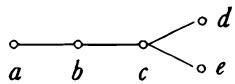
\includegraphics[keepaspectratio]{images/part001_959a1795.jpg}}

它表示一个图，其顶点为 \(a, b, c, d, e\)，其边为 \(\{a, b\}\)、\(\{b, c\}\)、\(\{c, d\}\) 和 \(\{c, e\}\)。

\appendixitem{图的连通分支}

设 \(\Gamma = (\mathbf{A},\mathbf{S})\) 是一张图。若 \(a\) 和 \(b\) 是两个顶点，则连接 \(a\) 和 \(b\) 的路是顶点序列 \((x_0,\ldots ,x_n)\)，属于图 \(\Gamma\)，满足 \(x_0 = a,x_n = b\)，且顶点 \(x_{i}\) 和 \(x_{i + 1}\) 在 \(0\leqslant i < n\) 时相连；整数 \(n\geqslant 0\) 是该路的长度。路 \((x_0,\ldots ,x_n)\) 称为单射的，当 \(x_{i}\neq x_{j}\) 对 \(i\neq j\) 成立。若路 \((x_0,\ldots ,x_n)\) 连接 \(a\) 和 \(b\)，且在这类路中长度最小，则它必为单射的；否则就存在 i 和 j，满足 \(0 \leqslant i < j \leqslant n\) 且 \(x_{i} = x_{j}\)，于是序列

\[
\left(x _ {0}, \dots , x _ {i}, x _ {j + 1}, \dots , x _ {n}\right)
\]

则会是一条连接 a 和 b 的长度为 \textless{} n 的路。

两个顶点 a 和 b 之间的关系 ``存在一条连接 a 和 b 的路'' 是 \(\Gamma\) 的一个等价关系 R，它定义在顶点集合 S 上。R 的等价类称为 \(\Gamma\) 的连通分支；如果 S 至多有一个连通分支，即 \(\Gamma\) 的任意两个顶点之间至少可以连一条路，则称 \(\Gamma\) 是连通的。

命题 1. 设 \(\Gamma = (A, S)\) 是一张图，\((S_{\alpha})_{\alpha \in L}\) 是它的连通分支族。记 \(\Gamma_{\alpha}\) 为 \(\Gamma\) 的满子图，其顶点集合为 \(S_{\alpha}\)。

\begin{enumerate}
\def\labelenumi{(\roman{enumi})}
\item
  对于 L 中任意 \(\alpha\)，图 \(\Gamma_{\alpha}\) 是连通的。
\item
  若 \(\Gamma' = (A', S')\) 是 \(\Gamma\) 的连通子图，则存在 L 中的 \(\alpha\)，使得 \(\Gamma' \subset \Gamma_{\alpha}\)。
\item
  若 \(\alpha \neq \beta\)，则 \(S_{\alpha}\) 的任何元素都不与 \(\Gamma\) 中 \(S_{\beta}\) 的任何元素相连（等价地，\(\Gamma\) 的每条边都是某个 \(\Gamma_{\alpha}\) 的边）。
\item
  设 \((\mathrm{S}_{\lambda}^{\prime})_{\lambda \in \mathbb{M}}\) 是 \(S\) 的一个划分，且若 \(\lambda \neq \mu\)，则 \(\mathrm{S}_{\lambda}^{\prime}\) 的任何元素都不与 \(\Gamma\) 中的 \(\mathrm{S}_{\mu}^{\prime}\) 的任何元素相连；则每个集合 \(\mathrm{S}_{\lambda}^{\prime}\) 都是 \(\Gamma\) 的连通分支的并集。
\item
  设 \(\alpha\) 属于 L，且 \(a\) 和 \(b\) 属于 \(S_{\alpha}\)。则存在一条路 \(c = (x_0, \ldots, x_n)\)，连接 \(a\) 和 \(b\)，位于 \(\Gamma\) 中。对于任意 \(i\)，满足 \(0 \leqslant i \leqslant n\)，路 \((x_0, \ldots, x_i)\) 连接 \(a\) 和 \(x_i\)，位于 \(\Gamma\) 中，所以 \(x_i \in S_{\alpha}\)。因此，\(c\) 是 \(\Gamma_{\alpha}\) 中连接 \(a\) 和 \(b\) 的一条路。由此 \(\Gamma_{\alpha}\) 是连通的。
\item
  设 \(\Gamma' = (A', S')\) 是 \(\Gamma\) 的一个非空连通子图，设 \(a\) 是 \(S'\) 的一个元素，且 \(S_{\alpha}\) 是 \(S\) 中包含 \(a\) 的连通分支。对于任意 \(b\)，它属于 \(S'\)，存在一条路 \(c\)，连接 \(a\) 和 \(b\)，位于 \(\Gamma'\) 中，从而 \(a\) 更不用说也位于 \(\Gamma\) 中。由此 \(S' \subset S_{\alpha}\)。
\item
  给定不同的元素 \(\alpha\) 和 \(\beta\)，它们属于 \(L\)，以及顶点 \(a \in S_{\alpha}\) 和 \(b \in S_{\beta}\)，不存在连接 \(a\) 和 \(b\) 的路，特别地，不存在连接 \(a\) 和 \(b\) 的边。
\item
  设 \(a\) 属于 \(S_{\lambda}'\)，且 \(S_{\alpha}\) 是 \(\Gamma\) 的连通分支，包含 \(a\)。于是，对于任意 \(b\)，它属于 \(S_{\alpha}\)，存在一条路 \((x_0, \ldots, x_n)\)，连接 \(a\) 和 \(b\)，位于 \(\Gamma\) 中。若 \(i\) 是满足 \(0 \leqslant i < n\) 的整数，且 \(x_i \in S_{\lambda}'\)，则 \(x_{i+1} \in S_{\lambda}'\)，因为 \(x_i\) 与 \(x_{i+1}\) 相连。由归纳法可知，\(x_i \in S_{\lambda}'\) 对 \(0 \leqslant i \leqslant n\) 成立，特别地，\(b = x_n\) 属于 \(S_{\lambda}'\)。因此，\(S_{\alpha} \subset S_{\lambda}'\)。
\end{enumerate}

推论 1. 图 \(\Gamma = (A, S)\) 连通，当且仅当不存在一个划分 \((S', S'')\)，将 \(S\) 分成两个非空子集，并且 \(S'\) 的任何元素都不与 \(\Gamma\) 中的 \(S''\) 的任何元素相连。

假设 \(\Gamma\) 不连通，并令 \(S'\) 为其一个连通分支。集合 \(S'' = S - S'\) 根据命题 1 (i) 是非空的，并且根据命题 1 (iii)，\(S'\) 的任何元素都不与 \(S''\) 的任何元素相连。

现在假设 \(\Gamma\) 连通，并设 \((S', S'')\) 是具有所述性质的一个划分。根据命题 1 (iv)，集合 \(S'\) 包含至少一个连通分支，因此 \(S' = S\) 且 \(S'' = \varnothing\)，矛盾。

推论 2. 一个子集 \(S'\)（\(S\) 的子集）是连通分支的并集，当且仅当属于 \(S'\) 的任何顶点都不与属于 \(S - S'\) 的任何顶点相连。

该条件由命题 1 (iv) 充分。由命题 1 (iii)，该条件也是必要的。

